%% 
%% Paper Template for the 7th International Symposium on Space Sailing (ISSS 2025)
%% 
%% This template is based on Elsevier's article class elsarticle.sty
%%
%% More on this class: https://www.elsevier.com/authors/author-schemas/latex-instructions
%% 
%% Version 1.0 (03 February 2025)
%%

\documentclass[final,3p,times,twocolumn]{elsarticle}

% \makeatletter % This is required to remove the footnote
% \def\ps@pprintTitle{%
%  \let\@oddhead\@empty
%  \let\@evenhead\@empty
%  \def\@oddfoot{}%
%  \let\@evenfoot\@oddfoot}
% \makeatother

\makeatletter
\def\ps@pprintTitle{%
  \let\@oddhead\@empty
  \let\@evenhead\@empty
  \def\@oddfoot{\thepage}% ← add page number here
  \let\@evenfoot\@oddfoot
}
\makeatother


\usepackage[utf8]{inputenc}
\usepackage{amsmath,amssymb}
\usepackage{siunitx}
\usepackage{hyperref}
\usepackage{booktabs,multirow}
\usepackage{float}
\usepackage{tabularx}
\usepackage{stfloats}
\usepackage{titlesec}
\usepackage[switch]{lineno}
\usepackage{etoolbox}
\usepackage{natbib}
\titlespacing{\subsection}{0pt}{*0.1}{*0.0} 

\bibliographystyle{abbrvnat.bst} 
\setcitestyle{authoryear}


% Turn on line numbering inside abstract
%\AtBeginEnvironment{abstract}{\linenumbers}

% Turn off line numbers in bibliography
%\AtBeginEnvironment{thebibliography}{\nolinenumbers}

\usepackage{fancyhdr} % To have custom headers
\usepackage{graphicx} % To include images



% Redefine title fontsize to match Word template
\makeatletter
\def\title#1{\gdef\@title{\fontsize{18pt}{22pt}\selectfont #1}}
\makeatother

% Adjust margins to match Word template
\geometry{top=2.17cm}

% Adjust header dimensions to match Word template
\setlength{\headheight}{3.5cm} 
% Set space between header and main text to zero
\setlength{\headsep}{0cm}   

% Create style for first page (which has the logo)
% \fancypagestyle{firstpage}{%
% \fancyhf{} % Clear all header and footer fields
% \lhead{\hspace*{-0.45cm} % Moves the logo -0.45 from the left margin
%     \raisebox{-0.6cm}{
\includegraphics[height=2.36cm]{ISSS_2025_Emblem_CMYK.pdf}}
%     }
% \chead{    
% \parbox[][2.25cm][t]{\textwidth}{\centering 7\textsuperscript{th} International Symposium on Space Sailing (ISSS 2025) \\ 
%     Delft, The Netherlands, 30 June – 4 July 2025
%     }}
% % Remove the horizontal line in the header
% \renewcommand{\headrulewidth}{0pt}}

\fancypagestyle{firstpage}{%
  \fancyhf{} % Clear all header and footer fields
  \lhead{\hspace*{-0.45cm}{\raisebox{-0.6cm}{
\includegraphics[height=2.36cm]{ISSS_2025_Emblem_CMYK.pdf}}}}
  \chead{
    \parbox[][2.25cm][t]{\textwidth}{\centering
      7\textsuperscript{th} International Symposium on Space Sailing (ISSS 2025) \\
      Delft, The Netherlands, 30 June – 4 July 2025
    }
  }
  \fancyfoot[C]{\thepage} % ← this adds the page number
  \renewcommand{\headrulewidth}{0pt}
}


% Define the custom header with centered text 1.25cm from top (3.5-1.25 = 2.25)
% \fancypagestyle{otherpages}{%
% \fancyhf{} % Clear all header and footer fields
% \chead{    
% \parbox[][2.25cm][t]{\textwidth}{\centering 7\textsuperscript{th}  International Symposium on Space Sailing (ISSS 2025) \\ 
%     Delft, The Netherlands, 30 June – 4 July 2025
%     }}
% % Remove the horizontal line in the header
% \renewcommand{\headrulewidth}{0pt}}
% \pagestyle{otherpages}

\fancypagestyle{otherpages}{%
  \fancyhf{}
  \chead{
    \parbox[][2.25cm][t]{\textwidth}{\centering
      7\textsuperscript{th} International Symposium on Space Sailing (ISSS 2025) \\
      Delft, The Netherlands, 30 June – 4 July 2025
    }
  }
  \fancyfoot[C]{\thepage} % ← add this line too
  \renewcommand{\headrulewidth}{0pt}
}

%\journal{Advances in Space Research}

\setlength{\footskip}{50pt}   % default ≈ 10–12pt, increase to push number lower

\begin{document}
%\linenumbers

\pagenumbering{arabic}


%\layout

\begin{frontmatter}

% \title{High-Altitude And LEO Testing Of The First Interstellar CubeSat Powered By Solar Sailing Technology (ISSS 2025)}

\title{Feasibility of Passive SMA Gain in LEO: Simulation and Stratospheric Demonstration of a Solar Sail CubeSat}

\author[1]{Matthew Acevski\corref{cor}}
\author[2]{Shiki Vaahan}
\author[2]{Piotr Fil}
\author[3]{Herbie Christophers}
\author[2]{Debdut Sengupta}
\author[2]{Fatima Sajid}
\author[1]{Madhav Rajeswar}
\author[4]{Ian Poon}
\author[1]{Rajveer Daga}
\author[5]{Neil Pakrasi}
\author[6]{Defne Ertugrul}



\address[1]{Department of Physics, Imperial College London, London, UK}
\address[2]{Department of Aeronautics, Imperial College London, London, UK}
\address[3]{Department of Mechanical Engineering, Imperial College London, London, UK}
\address[5]{Department of Electrical Engineering, Imperial College London, London, UK}
\address[6]{Department of Chemical Engineering, Imperial College London, London, UK}
\address[4]{Department of Bioengineering, Imperial College London, London, UK}

\cortext[cor]{Corresponding author, \href{mailto:matthew.acevski19@imperial.ac.uk}{matthew.acevski19@imperial.ac.uk}}

    
\begin{abstract}
\begin{linenumbers}
Project Svarog is a student-led initiative based out of Imperial College London aiming to reach the heliopause using solar sail technology. The sail will be passively spin-stabilised and would not require gravity assists unlike previous interplanetary missions which makes deep space exploration significantly more feasible. The project is at a stage where we have developed and tested our first fully integrated mechanical prototype on the European Space Agency's BEXUS program (Balloon EXperiment for University Students), which allowed us to test deployment and rotation of the prototype in both near-vacuum conditions and extreme temperatures as well as validate our flight hardware. We also aimed to validate a scaling law (highlighted in \cite{isss1}) for the behaviour of the sails under the influence of gravity. However, we were unable to complete this objective due to incomplete deployment of our sail on the BEXUS flight. Further, we have developed a high-fidelity comprehensive solar sail propagator model incorporating solar radiation pressure (SRP) and gravity-gradient torques - this model was developed to test the feasibility of trajectories for future launches into Low Earth Orbit (LEO) and interplanetary travel. In this paper, we discuss the developments and results of our orbital simulations as well as innovations in mechanical design made during the development of our BEXUS prototype in preparation for a future LEO or interplanetary mission.
\end{linenumbers}

\end{abstract}

\begin{keyword}
Deep Space \sep CubeSat \sep Solar Sail \sep Orbital Mechanics \sep Space Mechanisms 
\end{keyword}

\end{frontmatter}
\linenumbers

\thispagestyle{firstpage}



\section*{Nomenclature}

\def\arraystretch{1.5}
\begin{tabularx}{\linewidth}{l X}
$BEXUS$ & Balloon Experiment for University Students \\
$ESA$ & European Space Agency \\
$SSC$ & Swedish Space Corporation \\
$LEO$ & Low Earth Orbit \\
$SRP$ & Solar Radiation Pressure \\
$\mathbf{a}_{\text{SRP}}$ & Spacecraft acceleration due to SRP \\
$P_{\text{1 AU}}$ & SRP Flux at 1 AU \\
$C_r$ & Solar Sail Reflectivity Coefficient \\
\end{tabularx}
\begin{tabularx}{\linewidth}{l X}
$\boldsymbol{\tau}_{\text{SRP}}$ & Torque on Spacecraft due to SRP \\
$\mathbf{r}_{\text{lever}}$ & Vector from Centre of Mass to Centre of Pressure \\
$\mathbf{F}_{\text{SRP}}$ & Force on Spacecraft due to SRP \\
$\mathbf{a}_{\text{drag}}$ & Spacecraft acceleration due to drag \\
$C_d$ & Drag Coefficient \\
$\rho$ & Atmospheric Density \\
$\tau_{\text{gg}}$ & Torque from Gravitational Gradient \\
$\mu$ & Earth's Gravitational Parameter \\
$\mathbf{R}(q)$ & Quaternion-based rotation matrix \\
$\mathbf{I}_{\text{body}}$ & Inertia Tensor of Spacecraft \\
$\omega_n$ & Spacecraft Nutation Frequency \\
\end{tabularx}

\def\arraystretch{1.0}

\section{Introduction}

\par\noindent Solar sailing is becoming an increasingly popular form of propulsion. With the activities which are being conducted by JAXA during their IKAROS mission and subsequently during the development of OKEANOS and currently PIERIS, numerous aspects of solar sailing missions are becoming better understood, thus making it far more accessible to student teams. There have been several missions aimed at proving the feasibility of de-orbiting a satellite using dragsails, which, with easier access to Low Earth Orbit (LEO), are becoming quite common in recent years. Despite this, missions to higher orbits, where drag is sufficiently low to enable solar sailing are still uncommon. For this reason, the goal of our team is to catch a launch opportunity which would enable flight to Earth orbit (above LEO) or interplanetary space. This would be a great step towards developing a CubeSat capable of conducting high delta-V missions to the outer Solar System or solar poles, with potential to enter escape trajectories from the Solar System. In preparation for such a mission, our team has developed a demonstration prototype, which flew on a stratospheric balloon as a part of the European Space Agency's (ESA's) BEXUS programme. Within the scope of this mission, the mechanical assembly would be tested, demonstrating deployment and spin-up capability for the future space missions. This mechanical design and integration is discussed in Section \ref{bexus_section}.
\vspace{5pt}
\par\noindent Further to our effort to send a solar sail into the outer solar system, we have developed an in-house solar sail orbital simulation which incorporates features such as Solar Radiation Pressure (SRP), gravity, and torque. This allows us to test a variety of orbits for both LEO testing and future extra-solar trajectories. In the future, this code will be verified against existing industry standard orbital simulations and improved based on our own mission requirements. The first real test of this simulation will likely be when we develop our first LEO satellite which we hope to complete within the next 3-4 years.


\section{Mission Concept and previous work}
\noindent Over the past few years there was a broad range activities conducted at Imperial College London aimed at developing a spin stabilized solar sails aimed at exiting the Solar System \citep{isss1,jbis}. Due to the fact that this project is developed by a student society, a large part of the effort is devoted towards making the design extremely cost effective. This drives the campaign to use opportunities provided as educational projects to offset the most expensive part of mission, which is mostly flight testing. For this purpose, participation in the BEXUS program was used as a means to test deployment in near vacuum conditions on a large scale. Similarly in the future, the project is set to rely on the opportunities suited for students to launch into space and potentially to apply as a secondary payload to missions outside of the Earth's gravitational influence. It was determined that the best approach to achieve this goal, is to run two parallel streams of development - one focused on developing in-house orbital propagator and the other centred around increasing know-how in both mechanical and electronic design.
\vspace{5pt}
\par\noindent To drive the requirements for both of the sections, high-level objectives had to be set, so that they are focused on the main interstellar mission:

\begin{center}
    \emph{\textbf{"Construct a spacecraft that will reach the Sun's escape velocity and the heliopause (assumed at 123 AU from the Sun) within 100 years from launch by using solar sail technology."}}
\end{center}

\noindent They are subsequently supported by the following secondary objectives:
    \begin{enumerate}
        \item \emph{Measure the trajectory of the craft up to 10 AU from the Sun and validate it against theoretical models;}
        \item \emph{Get a visual confirmation of deployment;}
        \item \emph{Carry a payload representing human ingenuity on board.}
    \end{enumerate}

\noindent As a stepping stone, a LEO technology demonstrator, which is aimed at testing crucial functionalities and verifying the models developed for the deep space mission. For this demonstration, following set of objectives is set:

\begin{enumerate}
        \item \emph{Establish telemetry link with satellite;}
        \item \emph{Get a visual confirmation of deployment;}
        \item \emph{Conduct spin up and confirm the dynamics.}
    \end{enumerate}

\noindent For the purpose of investigation of the mission concept, highly customizable propagator written in Julia was developed and used to conduct some preliminary simulations, which will be described in further sections.
\vspace{5pt}
\par\noindent To progress with development of both mechanical and electronic design, the team takes part in the ESA/SSC BEXUS programme, where participation in the high-altitude balloon mission is conducted to iteratively improve the CubeSat design in preparation before the space mission. It enables conducting deployment of large solar sails in near vacuum conditions, following the approach used by JAXA in preparation to IKAROS mission. For the mission, the following set of objectives can be set to maximize the information gained before the space mission.

\begin{enumerate}
        \item \emph{Conduct the deployment of the sail;}
        \item \emph{Conduct the spin up of the sail;}
        \item \emph{Verify the model of deployment in vacuum under gravity.}
    \end{enumerate}

\noindent So far, one attempt of deployment during balloon mission was conducted during BEXUS 34 flight, where two of the four booms did not fully deploy. This failure was narrowed down to the operation of the doors. A more CubeSat-focused design will be flown on BEXUS 36. 
\section{Orbital Simulation}
\subsection{Orbital Mechanics}\vspace{2pt}
\noindent\textbf{{Desire to Maintain SSO}}
%SSO for stable illumination conditions (Rajveer)
%More Final version Fatima, can put back anything from before 
\vspace{5pt}
\par\noindent For a low Earth orbit (LEO) mission, our primary objective would be to collect high-fidelity in-situ data to calibrate and refine our proprietary orbital propagator, with a particular focus on solar radiation pressure (SRP) and atmospheric drag modelling. This includes validating force models under realistic conditions and improving the accuracy of drag coefficients in the free-molecular regime.
\vspace{5pt}
\par\noindent A secondary objective is to demonstrate measurable semi-major axis (\( a \)) growth using purely passive attitude control, without active torquing mechanisms. This capability remains largely unproven in published literature, where most \( a \) growth demonstrations rely on active sail steering or continuous attitude control. Verifying that \( a \) gain is achievable through inertially-fixed, spin-stabilised configurations would represent a significant milestone. It would open the door to viable low-cost solar sail missions that avoid the complexity and failure modes of active control systems. If \( a \) growth proves infeasible, due to a high mass-to-area ratio at launch, our fallback objective is to study de-orbiting behaviour and evaluate passive drag-sail dynamics in the later mission phases. Nonetheless, \( a \) growth remains the central experimental target of the mission.

\vspace{5pt}
\par\noindent As it is a near-polar orbit the inclination is set to a function of \( a \) and is approximately 98°, depending on various launch altitudes.

\begin{table}[htbp]
\centering
\begin{tabular}{c|c}
\textbf{Altitude (km)} & \textbf{Required Inclination (°)} \\
\hline
600 & 97.92 \\
700 & 98.04 \\
800 & 98.17 \\
900 & 98.31 \\
\end{tabular}
\caption{Required inclination to maintain Sun-synchronous orbits (SSO) for circular orbits (\(e = 0\)) at selected altitudes.}
\label{tab:sso_inclinations}
\end{table}
\vspace{5pt}
\par\noindent SSOs rely on natural secular precession of the Right Ascension of the Ascending Node (RAAN or \( \Omega \)), primarily driven by Earth’s oblateness (the \( J_2 \) perturbation). The required RAAN precession rate to maintain Sun-synchronicity is:

\begin{equation}
\frac{d\Omega}{dt} \approx 0.986^\circ/\text{day}
\label{eq:RAANrate}
\end{equation}

\noindent The precession induced by the \( J_2 \) perturbation is given by:
\begin{equation}
\dot{\Omega}
  = -\frac{3}{2}\,J_2\,
      \left(\frac{R_{E}}{a\bigl(1-e^{2}\bigr)}\right)^{\!2}
      \sqrt{\frac{\mu}{a^{3}}}\,
      \cos i
\end{equation}

\noindent To achieve this required value whilst passively stabilised, an orbit with appropriate altitude and inclination must be chosen such that the \( J_2 \) induced precession matches the apparent motion of the Sun \citep{montenbruck2000}. In this mission, we considered a purely passive solar sail, meaning the spacecraft has no onboard attitude control system and is freely left in space. It relies on spin-stabilisation to maintain a fixed inertial orientation with respect to the ECI reference frame. This configuration significantly reduces complexity, power requirements, and failure modes, but also constrains the sail to a non-adjustable thrust direction throughout the mission.

\vspace{5pt}
\par\noindent To assess how solar radiation pressure (SRP) and atmospheric drag affect the evolution of the orbit, we employ the Gauss Variational Equations (GVEs), which describe the time evolution of classical orbital elements under the influence of small perturbing accelerations. A perturbing acceleration vector \( \vec{F} \) is decomposed in the local orbital frame into three orthogonal components: radial (\( F_R \)), transverse (\( F_T \)), and normal (\( F_N \)). The GVEs governing the evolution of semi-major axis \( a \), eccentricity \( e \), inclination \( i \), argument of perigee \( \omega \), and right ascension of the ascending node \( \Omega \), are given by:

\begin{equation}
\frac{da}{dt} = \frac{2a^2}{h} \left[ e \sin{\theta} \, F_R + (1 + e \cos{\theta}) \, F_T \right]
\label{eq:da}
\end{equation}
\begin{equation}
\frac{de}{dt} = \frac{\mu}{h} \left[ \sin{\theta} \, F_R + \left( \cos{\theta} + \frac{e + \cos{\theta}}{1 + e \cos{\theta}} \right) F_T \right]
\end{equation}
\begin{equation}
\frac{di}{dt} = \frac{r \cos{u}}{h} \, F_N
\label{eq:di}
\end{equation}
\begin{equation}
\frac{d\Omega}{dt} = \frac{r \sin{u}}{h \sin{i}} \, F_N
\label{eq:domega}
\end{equation}

\par\noindent where \( h = \sqrt{\mu a (1 - e^2)} \) is the specific angular momentum, \( r = a(1 - e^2)/(1 + e \cos{\theta}) \) is the instantaneous orbital radius, \( \theta \) is the true anomaly, and \( u = \omega + \theta \) is the argument of latitude. All quantities are expressed in the ECI reference frame. A detailed derivation and discussion of the Gauss Variational Equations can be found in \cite{vallado2007}.

\vspace{5pt}
\noindent The expressions above are valid for general elliptical orbits and are particularly useful in identifying how each component of the perturbing acceleration affects specific orbital elements. In later sections, these equations are evaluated under mission-specific conditions to quantify the impact of SRP and drag on Sun-synchronous orbit maintenance and \( a \) evolution.

\vspace{5pt}
\par\noindent The equations above highlight that the semi-major axis (\( a \)) is primarily affected by the in-plane force components (\( F_R \) and \( F_T \)), which add or remove orbital energy and thereby modulate \( a \). In contrast, inclination (\( i \)) and RAAN (\( \Omega \)) evolve due to out-of-plane forces (\( F_N \)), which act normal to the orbital plane. Importantly, the secular RAAN precession required for Sun-synchronicity is inherently driven by Earth’s oblateness (\( J_2 \)), which introduces a persistent normal component to the gravitational field. This \( J_2 \)-induced term is already baked into the required value of \( \dot{\Omega} \approx 0.986^\circ/\text{day} \).

\vspace{5pt}
\par\noindent Consequently, to maintain this precession passively, any additional out-of-plane perturbations, such as those from solar radiation pressure (SRP) or atmospheric drag, must remain small compared to the \( J_2 \) contribution (i.e., \(|\dot{\Omega}_{\text{SRP}}| \ll |\dot{\Omega}_{J_2}|\)). Otherwise, they risk disrupting the balance required to preserve a stable Sun-synchronous orbit. Absent such external torques, both \( i \) and \( \Omega \) evolve predictably under the conservative \( J_2 \) dynamics.

\vspace{5pt}
\par\noindent Therefore, to maintain an SSO the out-of-plane \( F_N \) must be minimised. However, complete elimination is impossible in a spin-stabilised solar sail due to the secular precession of the orbital plane and the inertial nature of the sail's attitude. As the Earth progresses in its orbit, the Sun vector rotates by \(0.986^\circ\) per day (Eq~\eqref{eq:RAANrate}), causing the sail’s cone angle relative to the Sun to drift. This results in an increasing projection of the SRP and drag forces onto the out-of-plane direction.

\vspace{5pt}
\par\noindent Although solar-radiation-pressure (SRP) and atmospheric drag accelerations are weak, the normal components, \( F_N \), grow gradually as the orbital plane precesses and the sail’s cone angle drifts.  For the first \( \sim30 \) days this build-up is negligible: the external torques remain an order of magnitude below the \( J_2 \)-driven precession term, the attitude is quasi-steady, and we can confidently meet the mission’s data-collection objective.  Figure~\ref{fig:transversework} supports this, showing that the transverse work done by SRP stays high until day 30 and then falls off sharply.  Beyond that point the sail feathers toward an edge-on orientation; by \( \sim 3 \) months (after \( \sim 90^\circ \) of orbital-plane precession) the out-of-plane acceleration becomes difficult to characterise with the present model, and the resulting perturbation of \( i \) and \( \Omega \) is left to future study.

\vspace{5pt}
\par\noindent Furthermore, from Equation~\eqref{eq:da}, \( F_T \) is the most influential component to increase \( a \). This supports the intuitive determination that applying thrust in the direction of motion will add orbital energy. \( F_R \) also contributed to an increase in \( a \) in eccentric orbits however its effectiveness is dependent on phase and as a result is typically negligible in low-eccentricity LEO SSO. Therefore, in order to increase \( a \) whilst maintaining SSO the optimal configuration is to eliminate \( F_N \) to preserve RAAN and keep thrust aligned within the orbital plane. The orbital plane then becomes the ideal plane for thrust and the sail normal must be within it, any deviation from this ideal plane will introduce unwanted coupling between orbital energy gain and orbital geometry distortion. The only degree of freedom remaining with regards to sail orientation is the pitch angle (\( \alpha \)) which defines the angle between the sail normal and the Sun vector.

%Add a few line with citations supporting the above and expand reasons
%Talk about precession of RAAN for constant sun-line for satellite
%Another 150-200 words




%In this study, we analyse various Sun-synchronous orbits for our solar sail. 

%A sun-synchronous orbit is chosen to stabilise  
\vspace{5pt}
\par\noindent This modular Julia-based simulation framework models the coupled translational and rotational motion of a spacecraft using a 13-dimensional state vector: 6 components for position and velocity, 4 for attitude represented via quaternions, and 3 for body-frame angular velocities. Quaternion-based attitude propagation avoids gimbal lock and enables stable long-term integration of rotational dynamics. The framework aggregates all active force and torque contributions including solar radiation pressure, atmospheric drag, Earth's oblateness, albedo reflections, and central gravity, and numerically integrates the full system using a fixed time-step implementation of the Tsitouras 5/4 Runge–Kutta method \citep{tsitouras2011}. This ensures consistent step sizes across the simulation, supporting high-fidelity analysis of both orbital evolution and spacecraft attitude under sustained perturbations.
\vspace{7pt}

\noindent\textbf{SRP Force and Torque} \vspace{2pt}

\par\noindent The SRP model originates from photon momentum transfer on the sail. For a specular reflective square plate, the acceleration magnitude must account for angular dependence: McInnes (1999) shows the ideal flat-plate force scales as \( \cos^2{\alpha} \) relative to the Sun line \citep{mcinnes1999}. Our implementation uses:

\begin{equation}
    \mathbf{a}_{\text{SRP}} = \frac{P_{1\ \text{AU}} \, A \, C_r}{m c} \cos^2{\alpha} \, \hat{\mathbf{r}},
    \label{eq:srp_force}
\end{equation}

\par \noindent where $P_{1\ \text{AU}}$ represents the solar radiation pressure flux at one astronomical unit, $A$ is the sail’s effective reflective area, $C_r$ is the reflectivity coefficient, $m$ is the spacecraft mass, and $\hat{\mathbf{r}}$ is the unit vector pointing from the spacecraft toward the Sun \citep{torque_models}. This is computed in the inertial frame by retrieving the vector from the spacecraft to the Sun via SPICE. 
\vspace{5pt}
\par\noindent To handle solar eclipses, we implement a smoothed penumbra-aware shadow function using a hyperbolic tangent (tanh) transition model, which allows the SRP force to decrease gradually from full sunlight to complete shadow. This avoids discontinuities and numerical stiffness associated with binary shadow models. This technique follows the formulation in \cite{shadow} and is widely used in orbit propagators like GMAT and Orekit. Here, the shadow factor \( s \) is computed from the angle between the Sun and Earth as seen from the spacecraft,

\begin{equation}
s = \frac{1}{2} \left[ 1 + \tanh{\left( k \left( \frac{\theta - \theta_{\text{umbra}}}{\theta_{\text{penumbra}} - \theta_{\text{umbra}}} \right) \right)} \right],
\end{equation}

\noindent where \( \theta \) is the angle between the Sun and Earth as seen from the spacecraft, and \( k \) is a steepness factor controlling the transition sharpness \citep{shadow}. It was empirically chosen to be 15 to balance computational stability with physical accuracy, consistent with values chosen in literature (\( k \) = 10–20) \citep{shadow}. The resulting SRP acceleration becomes:

\begin{equation}
\mathbf{a}_{\text{SRP}}^{\text{shadowed}} = s \cdot \mathbf{a}_{\text{SRP}},
\end{equation}

\noindent ensuring a continuous and physically accurate reduction in SRP force during eclipses \citep{shadow}.

\vspace{5pt}
\par\noindent When the centre of pressure isn't aligned with the centre of mass, a SRP torque is also induced, given by,

\begin{equation}
    \boldsymbol{\tau}_{\text{SRP}} \: = \: \mathbf{r}_{\text{lever}} \: \times \: \mathbf{F}_{\text{SRP}},
    \label{eq:srp_torque}
\end{equation}

\noindent where \(\mathbf{F}_{\text{SRP}} = m \cdot \mathbf{a}_{\text{SRP}}\) \citep{torque_models}. The SPICE vector retrieved previously is now projected onto the body frame for this computation. The lever arm is in the body frame, while the SRP force is in the inertial frame and must be rotated. \vspace{7pt}

\noindent\textbf{Atmospheric Drag and Torque}\vspace{2pt}
\par\noindent In LEO, particularly below 800 km altitude, atmospheric drag acts in opposition to the spacecraft’s velocity relative to the co-rotating atmosphere. For computational efficiency and accuracy, we implement a piecewise-exponential density model fitted to U.S. Standard Atmosphere (1976) data from Braeunig’s atmospheric table \citep{braeunig_atmos}. In each altitude region \( i \), defined by breakpoints between 600–900 km, density is calculated as:

\begin{equation}
\rho(h) = \rho_0^{(i)} \exp\left(-\frac{h - h_0^{(i)}}{H^{(i)}}\right)
\label{eq:atmospheric_density}
\end{equation}

\noindent This approach captures the true density variation within 5\%  error while preserving runtime performance, compared to querying full MSIS models.
\vspace{5pt}
\par\noindent Aerodynamic forces use the free-molecule flow model with Sentman coefficients, \citep{sentman1961nasa} derived from the spacecraft’s angle-of-attack \( \alpha \):

\begin{align}
S &= \sin{\alpha}, \quad C = \cos{\alpha} \\
C_n &= (2 - \sigma) S C + \sigma \sqrt{\pi}\, S^2 \\
C_t &= \frac{2\sigma}{\sqrt{\pi}}\, S \\
C_D &= C_n S + C_t C \\
C_L &= C_n C - C_t S
\end{align}

\par\noindent Here, \( \sigma \) is the accommodation coefficient, typically set to 0.9 \citep{smith2019}. This matches our routine, converting angle-of-attack directly into drag (\( C_D \)) and lift (\( C_L \)) coefficients.

\vspace{5pt}
\par\noindent The drag plus lift acceleration vector is:

\begin{equation}
\mathbf{a}_{\mathrm{drag}} = \frac{A}{m} \cdot \frac{1}{2} \, \rho(h) \, \mathbf{v}_{\mathrm{rel}}^2 \left( -C_D \, \hat{\mathbf{v}}_{\mathrm{rel}} + C_L \, \hat{\mathbf{l}} \right)
\label{eq:drag_force}
\end{equation}

\noindent where \( \hat{\mathbf{l}} \) is the lift direction, normal to both relative velocity \( \mathbf{v}_{\mathrm{rel}} \) and the surface normal, and \( \mathbf{v}_{\mathrm{rel}} = \mathbf{v}_{\mathrm{ECI}} - (\boldsymbol{\omega}_E \times \mathbf{r}) \), with \( \boldsymbol{\omega}_E = [0,0,7.2921\times10^{-5}] \) rad/s.

\vspace{5pt}
\par\noindent The atmospheric drag torque around the centre-of-pressure (\( C_p \)), defined as the effective point of application of surface forces on the sail, (lever arm \( \mathbf{r}_{\text{lever}} \)) is then:

\begin{equation}
\boldsymbol{\tau}_{\mathrm{drag}} = \mathbf{r}_{\text{lever}} \times \left( m\,\mathbf{a}_{\mathrm{drag}} \right)
\label{eq:drag_torque}
\end{equation}

\par\noindent These algorithms are implemented directly within the simulation code, with separate routines handling the drag and lift calculation and the associated aerodynamic torque. The piece-wise exponential density fit together with the Sentman coefficients ensures accurate drag, lift and torque modelling across 600 – 900 km while keeping the simulation tractable. \vspace{7pt}

\noindent\textbf{Gravity Gradient Torque}\vspace{2pt}
\par\noindent Gravity gradient torque arises due to differential gravitational attraction across an extended body in orbit. This is particularly significant for elongated or asymmetric spacecraft such as solar sails, where the distance between the centre of mass and different points on the structure leads to non-uniform force distribution. The torque tends to align the spacecraft’s maximum inertia axis with the local vertical, acting as a passive attitude stabilizer.
\vspace{5pt}
\par\noindent Assuming a flat-plate structure for the sail, we model this effect by computing the torque in the body frame and rotating it into the inertial frame at each step. Here, we use \( \mathbf{R}(\mathbf{q}) \), the Direction Cosine Matrix (DCM) derived from the spacecraft's unit quaternion \( \mathbf{q} \), to implement this computation. The torque is given by the expression:
\begin{equation}
\boldsymbol{\tau}_{\text{gg}} = \frac{3\mu}{r^3} \cdot \mathbf{R}(\mathbf{q}) \left[ \left( \mathbf{R}(\mathbf{q})^\top \mathbf{r} \right) \times \left( \mathbf{I}_{\text{body}} \cdot \left( \mathbf{R}(\mathbf{q})^\top \mathbf{r} \right) \right) \right]
\end{equation}

\noindent where \(\mu\) is Earth's gravitational parameter, \(\mathbf{r}\) is the spacecraft's position vector in the inertial frame, and \(\mathbf{I}_{\text{body}}\) is the moment of inertia tensor expressed in the body-fixed frame \citep{grav_grad}. $\mathbf{I}_{\text{body}}$ was modelled as a diagonal matrix in the principal body frame, assuming symmetry about its main structural axes. We use the form:

\begin{equation}
\mathbf{I}_{\text{body}} = 
\begin{bmatrix}
I_{xx} & 0 & 0 \\
0 & I_{yy} & 0 \\
0 & 0 & I_{zz}
\end{bmatrix}.
\end{equation}

\noindent For the simulations, representative values \( I_{xx} = 15.0~\text{kg}\cdot\text{m}^2 \), \( I_{yy} = 15.0~\text{kg}\cdot\text{m}^2 \), and \( I_{zz} = 30.0~\text{kg}\cdot\text{m}^2 \) were chosen to reflect the geometry and mass distribution of the solar sail's cross-boom configuration. This simplification enables efficient computation of external torques without sacrificing fidelity under small-angle attitude variations.

\vspace{2pt}
\par\noindent High-fidelity attitude propagation was not the focus of this study and is deferred to future work. Instead, we assume the spacecraft is spin-stabilized about its principal axis, leading to steady inertial attitude behaviour over the timescales of interest. Justification for this assumption followed in the next section, where passive gyroscopic rigidity and the effect of environmental torques are assessed.

\vspace{5pt}
\par\noindent $\boldsymbol{\tau}_{\text{gg}}$ depends on attitude and position and is recomputed at every timestep. The maximum $\boldsymbol{\tau}_{\text{gg}}$ on the spacecraft occurs when its longest principal axis ($z$-axis) is orthogonal to the radial vector from the Earth to the spacecraft. This misalignment introduced a restoring torque that attempts to align the $z$-axis with the radial direction to minimise gravitational potential energy. This orientation maximizes the term $\mathbf{r}_{\text{body}} \times (\mathbf{I}_{\text{body}} \cdot \mathbf{r}_{\text{body}})$, producing the largest possible torque within the orbit. Consequently, the greatest magnitudes were observed when the spacecraft was perturbed away from this equilibrium alignment. The gravity-gradient torque is computed at every step by a dedicated routine and supplied to the numerical propagator alongside the other environmental torques.\vspace{5pt}


\par\noindent This formulation assumes a rigid spacecraft with known principal moments of inertia. The attitude quaternion \( \mathbf{q} \) evolves dynamically throughout the simulation, and \( \mathbf{R}(\mathbf{q}) \) is updated at each integration step to accurately reflect the body's orientation.

\vspace{5pt}
\par\noindent For a spacecraft with dimensions on the order of several meters and inertia values around \(1\text{–}10~\text{kg}\cdot\text{m}^2\), the magnitude of gravity gradient torque, \(\boldsymbol{\tau}_{\text{gg}}\), typically reaches \(10^{-7}\text{–}10^{-6}~\text{N}\cdot\text{m}\) in Low Earth Orbit (LEO). While relatively small in instantaneous magnitude, its persistent effect can induce measurable attitude drift or nutation over multi-Week timescales, particularly in the absence of active control. As evidenced in Table~\ref{tab:torque_summary}, simulations that account for external torques show small but non-negligible deviations in quaternion orientation \( \mathbf{q} \) and orbital position over 30 days, with gravity gradient torque identified as the dominant contributor.\vspace{5pt}


\noindent\textbf{Albedo Model} \vspace{2pt}

\par\noindent To capture the small but non-negligible effect of the sunlight reflected from Earth onto the spacecraft, we implement a Lambertian diffuse albedo model. This model approximates Earth as a spherical, uniformly reflecting body that scatters incoming radiation isotropically over the sunlit hemisphere. This radiation imparts momentum onto the spacecraft, similar to SRP, producing a force and torque when the \( C_P \) is offset from the \( C_G \). 
\vspace{5pt}
\par\noindent This acceleration is given by,
\begin{equation}
    \mathbf{a}_{\text{albedo}} \: = \: \frac{P_{\odot}\,a}{c}\,\left(\frac{R_E}{d}\right)^2\,\cos^2{\alpha}\,\frac{A}{m}\,\hat{\mathbf{n}},
\end{equation}

\noindent where \( P_{\odot} = 1361~\text{W}/\text{m}^2 \) is the solar constant, \( a = 0.3 \) is the Earth's albedo \citep{albedo}, \( R_E \) is the radius of the Earth, \( d \) is the earth to spacecraft distance, and \( \alpha \) is the angle between the sail normal \( \hat{\mathbf{n}} \) and the direction from Earth centre to spacecraft. Simulated accelerations results sit on the order of \( 10^{-7} \) m/s\(^2\) in LEO, which is comparable to SRP.

\vspace{5pt}
\par\noindent This also produces a corresponding torque given by,
\begin{equation}
    \boldsymbol{\tau}_{\text{albedo}} \: = \: \mathbf{r}_{\text{lever}} \: \times \: \mathbf{F}_{\text{albedo}},
\end{equation}

\noindent where $\mathbf{F}_{\text{albedo}} \, = \, m \, \cdot \mathbf{a}_{\text{albedo}}$. The albedo effect is represented as an additional perturbing force and torque pair within the propagator.
\vspace{5pt}
\par\noindent It is worth noting that this computation relies on a few heavy assumptions, such as ignoring the oblateness of the Earth in the Lambertian approximation, and constant uniform albedo over time and surface. \vspace{7pt}

\noindent\textbf{Validation and Model Fidelity: Comparison Between Analytical and Simulated Effects} \vspace{2pt}
\par\noindent To validate the correctness and consistency of our implemented perturbation models, we compare the net state evolution from simulations against analytical expectations derived from classical force magnitudes and orbital mechanics. These comparisons include absolute differences in position, velocity, quaternion orientation, and angular velocity over a 30-day period, also supported by \cite{smoothing}. Table~\ref{tab:torque_diff_only} outlines this comparison, using benchmark values derived from classical mechanics and solar sail literature.

\begin{table}[htbp]
\centering
\small
\begin{tabular}{p{3.5cm}p{3.0cm}}
\toprule
\textbf{Quantity} & \textbf{Absolute Difference} \\
\midrule
Quaternion ($\mathbf{q}$) & $\sim 10^{-5}$ \\
Angular velocity ($\boldsymbol{\omega}$) & $< 10^{-5}$\,rad/s \\
Position ($\mathbf{r}$) & $\sim 1.3$\,m \\
\bottomrule
\end{tabular}
\caption{Final-state comparison between torqued and torque-free runs over 30 days due to environmental torques.}
\label{tab:torque_diff_only}
\end{table}

\noindent The deviations between simulated and analytical values primarily stem from two factors. First, the finite time-step integration inherent in the \texttt{DifferentialEquations.jl} backend introduces minor numerical dispersion. Second, for orbit-to-orbit comparisons, orbital phase can amplify or attenuate the net perturbative effects over finite-time windows, particularly for \( \text{SRP} \) and drag, whose vector contributions vary over the orbit. Shadow modeling (binary eclipse inclusion) in \( \text{SRP} \) further causes step-wise force suppression, breaking strict continuity in some cases.

\begin{table}[H]
\centering
\renewcommand{\arraystretch}{1.3}
\setlength{\tabcolsep}{4pt} % tighter cell padding
\footnotesize
\begin{tabularx}{\linewidth}{@{}lccc@{}}
\toprule
\textbf{Torque} & \textbf{Included} & \textbf{Simulated (N$\cdot$m)} & \textbf{Analytical (N$\cdot$m)} \\
\midrule
SRP               & Yes & $1.0 \times 10^{-7}$       & $0$–$2 \times 10^{-6}$        \\
Atmos.\ Drag      & Yes & $3.9 \times 10^{-7}$       & $0$–$3 \times 10^{-7}$        \\
Gravity Gradient  & Yes & $2.7 \times 10^{-6}$       & $2$–$4 \times 10^{-6}$        \\
3rd Body Grav.    & No  & –                          & $\sim 10^{-8}$                \\
Relativity        & No  & –                          & $\sim 10^{-10}$               \\
Tidal (Moon)      & No  & –                          & $\sim 10^{-9}$                \\
\bottomrule
\end{tabularx}
\caption{Simulated vs.\ analytical torque magnitudes (N$\cdot$m) for included and excluded sources.}
\label{tab:torque_summary}
\end{table}


\begin{table}[H]
\centering
\renewcommand{\arraystretch}{1.3}
\setlength{\tabcolsep}{2pt}
\footnotesize
\begin{tabularx}{\linewidth}{lccc}
\toprule
\textbf{Force} & \textbf{Included} & \textbf{Simulated (m/s²)} & \textbf{Analytical (m/s²)} \\
\midrule
Earth Gravity         & Yes & $7.96$                   & $7.96$                   \\
\( J_2 \) Perturbation  & Yes & $3.2 \times 10^{-3}$    & $2$–$5 \times 10^{-3}$  \\
SRP                   & Yes & $1.2 \times 10^{-7}$    & $0$–$3.1 \times 10^{-6}$ \\
Atmos. Drag      & Yes & $0.8 \times 10^{-7}$    & $0$–$5 \times 10^{-6}$  \\
3rd Body Grav.    & No & —                       & $\sim 10^{-8}$       \\
Relativity  & No & —                       & $\sim 10^{-10}$     \\
\bottomrule
\end{tabularx}
\caption{Simulated vs. analytical force magnitudes (m/s²) for included and excluded perturbations.}
\label{tab:force_summary}
\end{table}


\par\noindent In terms of model justification, all non-negligible forces and torques over a 120 day horizon were included, as shown in Table \ref{tab:torque_summary} (verified in \cite{torque_lit}) and Table \ref{tab:force_summary}. The analytical \( \text{SRP} \) and drag torque/force values were calculated from the equations defined in the body previously, eqns. (\ref{eq:srp_force}), (\ref{eq:srp_torque}), (\ref{eq:drag_force}), \& (\ref{eq:drag_torque}). \( J_2 \) force analytical comparisons and third-body effects (from the Moon and Sun) were taken from \cite{j2force}. \( J_2 \) is significant and included in the simulation, while 3rd body acceleration is negligible, under \(10^{-8}~\text{m/s}^2\). Relativistic perigee precession contributes even smaller corrections at \(10^{-10}~\text{m/s}^2\), from \cite{relativityforce}. These are both 2–3 orders of magnitude below drag and \( \text{SRP} \), and show negligible cumulative influence within the time bounds studied. Even in heliocentric missions, relativity was very negligible at much higher velocities, which implies the same assumptions apply for our sail model in LEO \citep{isss1}. Hence, they were excluded to reduce computational overhead.

\vspace{5pt}
\par\noindent This comprehensive alignment between simulation and theory, both in scale and temporal behaviour, validates the chosen force model suite. Deviations remained low across all cases, and torques remained consistently within expected bounds across attitude axes. This confirms the correctness of both dynamic modelling and implementation.

\vspace{5pt}
\par\noindent Due to systemic constraints, our solar sail features solely passive attitude control. For our LEO test, our solar sail is spin stabilised about the sail normal. This follows the same treatment as IKAROS \citep{tsuda2013achievement}, which utilised this spin for sail deployment and structural and gyroscopic stability.

\vspace{5pt}
\par\noindent \par\noindent This helps the sail maintain a fixed orientation and makes it resistant to small external torques, which are especially significant in LEO with gravity gradient and drag being significant, in addition to SRP. This stability is further maintained due to the fact that any asymmetries in \( C_P \) simply result in periodic torque components aligned normally to the spin axis. These components rotate with the spacecraft over its orbit, and therefore nearly cancel out over the period, producing nutation (or precession) with minimal long-term reorientation \citep{TimeAvg}.  

\vspace{5pt}
\par\noindent
Since our external torques are low (as seen in Table \ref{tab:torque_summary}) and our spin rate is high, gyroscopic stiffness results in \( C_P \) being quasi-steady in the body frame. Therefore, torque from both SRP and drag can be approximated as periodic over an orbital cycle and would be negligible within our 120-day analysis time frame. Gravity Gradient would similarly only cause nutation within our interval.

\vspace{5pt}
\par\noindent
The above only holds true if the spacecraft is roughly axis-symmetric about the main axes (to prevent unbounded precession or nutation growth), resulting in a diagonal inertia tensor (\( \mathbf{I} \)).
The spin rate, \( \omega_z \), should also be sufficiently high \citep{SpinRate},


\begin{equation}
\omega_z \gg \sqrt{\frac{|\boldsymbol{\tau}|}{I_{zz}}}
\label{eq:SpinRate}
\end{equation}

\par\noindent \par\noindent \(C_P\) and Centre of Mass should be closely aligned along the spin axis to minimise spin-axis torque. Misalignment can lead to torque components that reduce angular momentum and gyroscopic stiffness, potentially causing drift of the spin axis, particularly when \(I_{xx}\) and \(I_{yy}\) are comparable. However, from the order-of-magnitude torques observed in Table~\ref{tab:torque_summary} and the principal moment of inertia \(I_{zz} = 30.0~\text{kg}\cdot\text{m}^2\), it is evident that a spin rate of 1.0~rad/s provides sufficient gyroscopic rigidity to maintain inertial attitude stability over the 120-day propagation interval.



\vspace{5pt}
\par\noindent The above are sufficiently met by our sail with a spin rate of 1.0~rad/s, a diagonal moment of inertia tensor, and minimal spin-axis torque due to external sources, owing to close alignment of \(C_P\) and the spin axis.

\vspace{5pt}
\par\noindent Therefore, with \(C_P\) almost collinear with the spin axis, the spacecraft behaves as a rigid spinner throughout the 120~day propagation. The nominal 1.0~rad~s$^{-1}$ spin supplies ample gyroscopic stiffness, so the environmental torques listed in Table~\ref{tab:torque_summary} merely excite small, bounded nutation. No secular drift of the spin axis is observed in the simulation, and the sail normal can be regarded as inertially fixed for the purpose of the force model validation.

% \vspace{7pt}
% \noindent \subsection{Attitude Stability Analysis over a 30--Day Window}\label{sec:att_stab}

% \par\noindent To assess whether the assumed spin rate is sufficient to maintain inertial stability, we quantify the cumulative effect of environmental torques over a representative 30-day interval. This interval corresponds to the early phase of the mission, during which predictable sail orientation is critical for achieving key objectives such as semi-major axis (\(a\)) gain and force model validation.

% \vspace{5pt}
% \par\noindent As shown in Table~\ref{tab:torque_summary}, the combined environmental torque, including gravity gradient, solar radiation pressure (SRP), and atmospheric drag, does not exceed \(\tau_{\max} \approx 2.7 \times 10^{-6}~\text{N}\cdot\text{m}\). While the gravity gradient torque is oscillatory and does not produce secular changes in the spin axis, it is the drag and SRP torques that can introduce small secular effects over time. Given a principal moment of inertia \(I_z = 7.5~\text{kg}\cdot\text{m}^2\), the corresponding maximum angular acceleration is:

% \begin{equation}
% \alpha_{\max} = \frac{\tau_{\max}}{I_z} = \frac{3.9 \times 10^{-7}}{30.0} \approx 1.2 \times 10^{-8}~\text{rad/s}^2.
% \end{equation}

% \par\noindent Assuming this worst-case torque acts continuously and coherently in the destabilizing direction, the accumulated angular deviation over 30 days is:

% \begin{equation}
% \begin{aligned}
% \Delta \theta &\approx \frac{1}{2} \alpha_{\max} t^2 
% = \frac{1}{2}(3.6 \times 10^{-7}) \cdot (60 \times 60 \times 24 \times 30)^2 \\
%               &\approx 0.172~\text{rad} \\
%               &\approx 9.85^\circ
% \end{aligned}
% \end{equation}

% \par\noindent While this appears significant, it represents a highly conservative upper bound. In practice, the spacecraft's 1.0 rad/s spin causes external torques to rotate in the body frame, effectively averaging out over each orbit. This results in bounded nutation rather than unbounded precession or drift.

% \vspace{5pt}
% \par\noindent Although gravity gradient torque dominates in magnitude, its effect is inherently oscillatory and varies periodically over the orbit. It reaches peak values at specific points when the principal axis aligns with the local gravity vector. While these peaks occur in opposite directions during each orbital cycle, the net contribution to long-term angular momentum change is minimal in spin-stabilized systems, as the oscillatory torque primarily induces bounded nutation rather than secular drift.

% \vspace{5pt}
% \par\noindent It is also worth noting that the orbital plane gradually precesses over time due to the \(J_2\) effect. This alters the inertial direction of the gravity gradient torque vector. However, analysing the long-term coupling between orbital precession and attitude drift is beyond the scope of this study. Our objective here is to confirm that the attitude remains sufficiently stable over the first month of operations for early design validation.

% \vspace{5pt}
% \par\noindent This analysis provides confidence that the sail’s inertial orientation will remain quasi-steady for at least 30 days, ensuring consistency in SRP and drag modelling and meeting the mission’s short-term requirements. Longer-term attitude behaviour may require refinement in future phases, particularly as asymmetric degradation or structural shifts become significant.

\vspace{10pt}
\noindent\textbf{Spin Stabilisation and Attitude Dynamics} \vspace{2pt}

\noindent The spacecraft is initialized with a nominal angular velocity of $\boldsymbol{\omega}_0 = [0,\,0,\,1.0]$~rad/s, corresponding to a spin about its body-fixed $z$-axis. This spin imparts gyroscopic stiffness to the system, passively stabilizing the attitude in the absence of active control. It also simplifies the net effect of non-conservative torques such as SRP and atmospheric drag, as these rotate in the body frame and tend to average out.

\vspace{5pt}
\par\noindent To maintain passive stability, the spacecraft uses a lightweight cross-braced sail structure that increases the moment of inertia about the spin axis ($I_{zz}$) without significantly affecting the transverse moments ($I_{xx}$, $I_{yy}$). This enhances gyroscopic stiffness, suppresses nutation, and limits coning motion. In our configuration, the inertia values are: 
\[
I_{zz} = 30.0~\text{kg}\cdot\text{m}^2,\quad I_{yy} = I_{xx} = 15.0~\text{kg}\cdot\text{m}^2
\]
ensuring near-axisymmetric behaviour. A key condition for passive spin stability is \citep{hubert2008}:

\begin{equation}
I_{zz} \gg I_{xx},\, I_{yy},
\end{equation}
which ensures that the spin angular momentum remains strongly aligned with the $z$-axis and resists external reorientation.

\vspace{5pt}
\par\noindent The dynamics of spin-stabilized rigid bodies are governed by Euler’s rotation equations \citep{goldsteinL13}:

\begin{equation}
\mathbf{I} \cdot \dot{\boldsymbol{\omega}} + \boldsymbol{\omega} \times (\mathbf{I} \cdot \boldsymbol{\omega}) = \boldsymbol{\tau}
\end{equation}

where $\boldsymbol{\tau}$ includes all environmental torques (SRP, drag, gravity gradient). For small perturbations, transverse angular rates $\omega_x$, $\omega_y$ exhibit bounded harmonic motion (nutation) with characteristic frequency \citep{hubert2008}:

\begin{equation}
\omega_n \approx \omega_z \cdot \sqrt{\frac{I_{zz} - I_{xx}}{I_{xx}}}
\end{equation}

\noindent With our current parameters and $\omega_z = 1.0$ rad/s, this yields:
\[
\omega_n \approx 1.0 \cdot \sqrt{\frac{30.0 - 15.0}{15.0}} \approx 1.0~\text{rad/s}, \quad
T_n = \frac{2\pi}{\omega_n} \approx 6.28~\text{s}
\]
\noindent This short-period nutation oscillation ensures fast energy redistribution, and the high $I_{zz}$ reduces coning amplitude.

\vspace{5pt}
\par\noindent To avoid long-term destabilization due to gravity-gradient torque, a minimum spin rate is also required. Analytical stability conditions from \cite{stability} state:

\begin{equation}
\omega_z \geq \sqrt{\frac{3\mu}{r^3} \cdot \frac{I_{xx}}{I_{zz}}}
\end{equation}
At our mission altitude (700–800 km), this gives:
\[
\omega_z \gtrsim 0.0013~\text{rad/s}, \quad T_{\text{max}} \approx \frac{2\pi}{\omega_z} \approx 80.6~\text{minutes}
\]
Our nominal value of $\omega_z = 1.0$ rad/s is therefore two orders of magnitude above the minimum threshold, ensuring robust attitude stability even under worst-case torques.

\vspace{5pt}
\par\noindent In addition to suppressing coning, spin stabilization also acts as a low-pass filter for transverse torques. We define a lever arm vector, $\mathbf{r}_{\text{lever}}$, connecting the center of pressure ($C_P$) to the center of mass ($C_G$). Any in-plane ($x$–$y$) misalignments result in periodic torque components that rotate with the spacecraft. These are symmetrically distributed over one revolution and are averaged out by the fast angular momentum vector. Consequently, such perturbations do not lead to secular drift in the transverse axes.

\vspace{5pt}
\par\noindent However, out-of-plane ($z$-axis) torque components are not filtered out in this way and can gradually alter spin rate or induce axial reorientation. Therefore, $\mathbf{r}_{\text{lever}}$ must be critically aligned along the spin axis ($z$-axis) and remain stable relative to attitude and structural deformation. This alignment is essential for maintaining long-term attitude predictability, especially over the first 30 days of mission.

\vspace{5pt}
\par\noindent Beyond this point, both attitude and orbital drift become increasingly significant. Secular changes to the \( a \) and \( i \), driven by drag and SRP, begin to distort the \( J_2 \)-induced \( \Omega \) precession rate. Concurrently, as the orbital plane precesses while the sail remains inertially fixed, a slow but accumulating out-of-plane (\( F_N \)) SRP force develops, further perturbing the orbit away from the ideal Sun synchronous configuration.

\vspace{5pt}
\par\noindent Since the coupled evolution of attitude and orbit becomes increasingly non-linear and mission-dependent beyond this regime, it is difficult to analytically guarantee stability or predict exact system behaviour. However, the objective at this design stage is not to quantify long-term performance with precision, but rather to confirm that our initial configuration provides stable and predictable dynamics during early mission operations. For this reason, a 30-day window is selected as a conservative horizon within which all subsystems remain within controllable and linear limits. Detailed assessment of long-term attitude-orbit coupling is left for future work. 

\vspace{7pt}
\subsection{Initial Trajectory Estimation (LEO)}

\par\noindent Given the above considerations, we are constrained to fixed-attitude sails with their normal vectors lying strictly within the orbital plane. Any out-of-plane component would generate cross-track accelerations, violating the planar dynamics assumption~\citep{mcinnes1999}. The sail normal is therefore restricted to a single in-plane angle, meaning that once we fix the semi-major axis (\( a \)) to manage drag, and allow inclination and eccentricity to follow from that, the only remaining free orbital parameter is the Right Ascension of the Ascending Node (\( \Omega \)).

\vspace{5pt}
\par\noindent Due to our constraint that the solar sail normal must remain within the orbital plane, the only available degree of freedom for attitude orientation at the moment of launch release is denoted by $\alpha$. This angle is defined as the in-plane angle between the sail normal vector and the local radial direction, measured positively in the direction of orbital motion.

\vspace{5pt}
\par\noindent To explore the sensitivity of orbital evolution to initial launch parameter, we conducted a two-dimensional parameter sweep over the following domain: 
\vspace{0pt}
 \[
 \mathcal{D}
   = \left\{\,(\mathrm{LTAN},\,\alpha) \in \mathbb{R}^{2} \;\middle|\;
         0 \le \mathrm{LTAN} < 24,\; 
         0^\circ \le \alpha \le 180^\circ \right\},
 \]
\noindent where LTAN is the Local Time of Ascending Node, expressed in hours, and $\alpha$ is expressed in degrees.

\par\noindent Each trajectory in this grid was propagated for 120 days (approximately 1500\,hrs), within this period the sail is expected to not build up significant $a_{\mathrm{N}}$. Therefore, SSO maintenance is expected for this duration.
\begin{figure}[htbp]
    \centering
    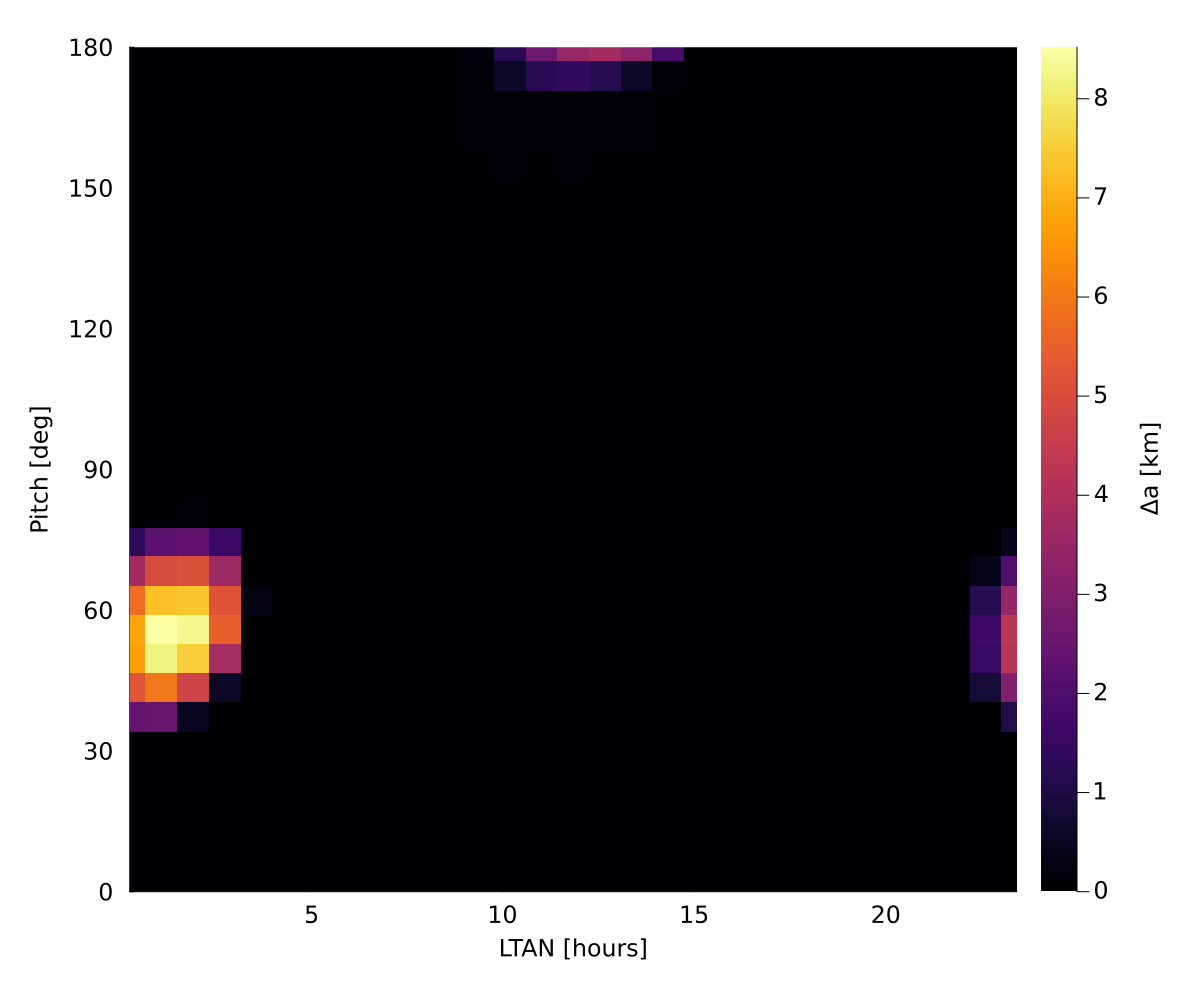
\includegraphics[width=1\linewidth]{figs/delta_a_heatmap_ltan.png}
    \setlength{\abovecaptionskip}{0pt}
    \caption{Heat-map of $\Delta a$ in search space}
    \label{fig:SMA_gain}
\end{figure}

\par\noindent Figure~\ref{fig:SMA_gain} highlights that LTANs near midnight conditions are crucial for achieving a positive \( \Delta a \). This finding aligns with physical intuition: such LTANs maximize the duration the sail spends within the Earth's umbra and penumbra regions, introducing a day--night asymmetry in SRP exposure. This asymmetry alters the effective SRP acceleration between the inbound and outbound legs of each orbit, where "inbound" refers to motion toward the Sun and "outbound" to motion away from it. In particular, the global optimum observed near a 01:30 LTAN leverages this asymmetry: the sail receives favourable SRP projection during the Sun-outbound leg, while SRP is partially suppressed by eclipse during the less favourable Sun-inbound leg. This configuration results in a net positive transverse work contribution from SRP over each orbit, as illustrated in Figure~\ref{fig:SRP work}, which depicts the work done during the first orbit. This cumulative effect enables gradual semi-major axis growth, despite the passive and spin-stabilized nature of the sail's orientation.

\vspace{5pt}
\par\noindent A secondary cluster of local optimum solutions is also observed near an LTAN of 12:00. However, in this region, the range of sail pitch angles that yield a positive \( \Delta a \) is significantly narrower. This indicates that the trajectory’s performance is more sensitive to small deviations in attitude, making it less robust under realistic uncertainties. In particular, the achievable precision in setting the sail’s inertial pitch angle at the moment of launch is currently unknown and likely limited by deployment dynamics and spin-up transients. In contrast, the region around the global optimum near 01:30 exhibits a broader and more forgiving band of favourable attitudes. For this reason, the candidate solution set for further analysis was selected from this more robust region, where performance is less vulnerable to pitch angle initialization errors and modelling imperfections.

\vspace{5pt}
\noindent Another important observation is that the only regions within the search space that fail to produce any net gain in semi-major axis are those near terminator orbits, where the LTAN is around 06:00 or 18:00 LTAN. In these configurations, the sail remains almost continuously illuminated and never significantly enters the Earth's penumbra. As a result, it cannot exploit the asymmetry in SRP exposure between the Sun-inbound and Sun-outbound legs. Furthermore, the constraint that the sail normal must lie within the orbital plane leads to negligible transverse acceleration (\( a_{\mathrm{T}} \approx 0 \)) in these geometries. Although long-term orbital precession can eventually produce some transverse SRP force, the resulting impulse builds up too slowly to meaningfully counteract atmospheric drag. Consequently, these LTAN regions are ineffective for achieving sustained orbital energy gain.

\begin{figure}[htbp]
    \centering
    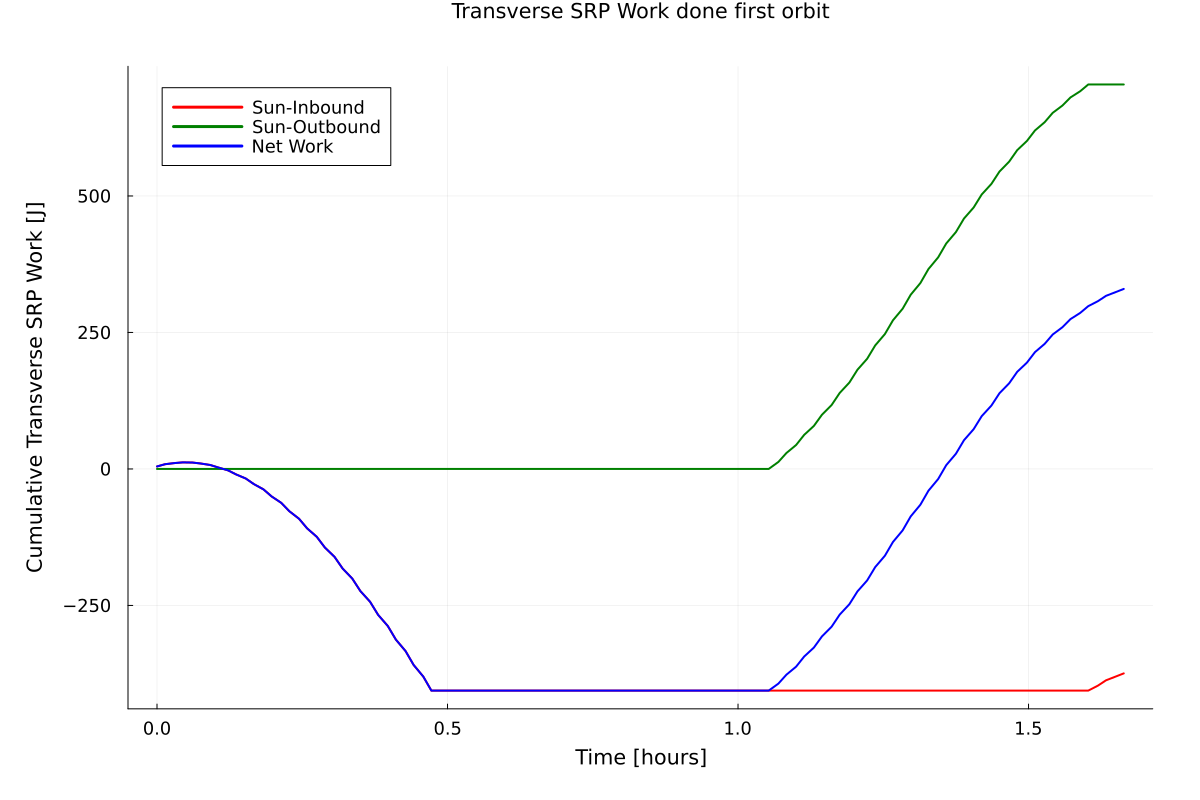
\includegraphics[width=1\linewidth]{figs/srp_tranversework.png}
    \setlength{\abovecaptionskip}{0pt}
    \caption{Transverse Work Done by SRP During First Orbit Post-Launch}
    \label{fig:SRP work}
\end{figure}
\vspace{5pt} 
\par\noindent Figure~\ref{fig:SRP work} illustrates the cumulative transverse SRP work performed over a single orbit for the candidate trajectory launched near the global optimum LTAN of 01:30. Notably, between approximately 0.5 and 1.0 hours after perigee passage, corresponding to the latter two-thirds of the Sun-outbound leg, the spacecraft enters the Earth's umbra. During this phase, SRP is effectively suppressed due to shadowing, while the Sun-inbound leg remains mostly illuminated. This induces a significant asymmetry in SRP exposure over the orbit.

\vspace{5pt}
\par\noindent As a result, the net transverse work done by SRP becomes strongly positive each orbit: the sail receives substantial transverse acceleration during the illuminated outbound segment, while minimal opposing acceleration is applied during the shadowed inbound segment. This asymmetry in work accumulation drives the observed growth in \( a \), even under a passive, spin-stabilized configuration with fixed inertial pitch. The evidence supports the earlier physical intuition, that eclipse driven modulation of SRP can be leveraged to enable net orbital energy gain despite the absence of active attitude control.

\begin{figure}[htbp]
    \centering
    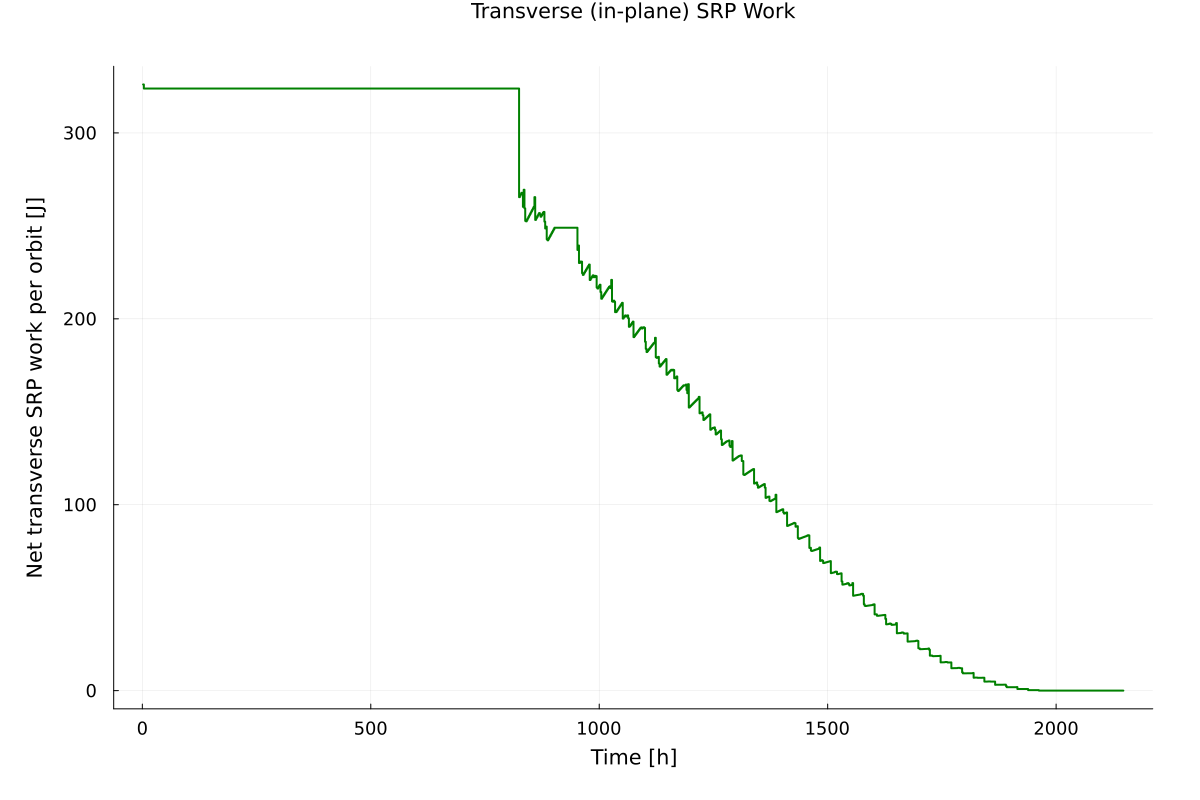
\includegraphics[width=1\linewidth]{figs/transversework.png}
    \setlength{\abovecaptionskip}{0pt}
    \caption{Work done per orbit in transverse (RTN) direction by SRP in first 3 months}
    \label{fig:transversework}
\end{figure}

\vspace{5pt}
\par\noindent 
Figure~\ref{fig:transversework} shows that the work performed by solar radiation pressure in the transverse (RTN) direction falls off sharply after the first month, reinforcing our choice of a \(30\)\,day window as the most reliable period for quasi–SSO behaviour.  Owing to spin stabilisation, the sail’s spin axis remains inertially fixed, while the orbital plane precesses secularly.  After \(\sim90^\circ\) of precession, about \(3\)\ months, the sail has effectively rotated from face-on to edge-on with respect to the Sun, so its projected area (and hence SRP cross-section) approaches zero.  This ``near-feathered’’ state keeps out-of-plane perturbations small and passively preserves Sun-synchrony, but it also curtails further semi-major-axis growth.

\vspace{5pt}
\par\noindent To ensure that a meaningful increase in \(a\) is achieved before the sail feathers, or before secondary effects such as eccentricity drift, atmospheric drag, or attitude jitter dominate, we impose the requirement that the time to reach the maximum semi-major-axis change, \(t_{\Delta a_{\mathrm{max}}}\), must occur within the first three months.  Satisfying this constraint guarantees that the candidate trajectory delivers its peak performance while quasi-SSO conditions remain robust.



\begin{figure}[htbp]
    \centering
    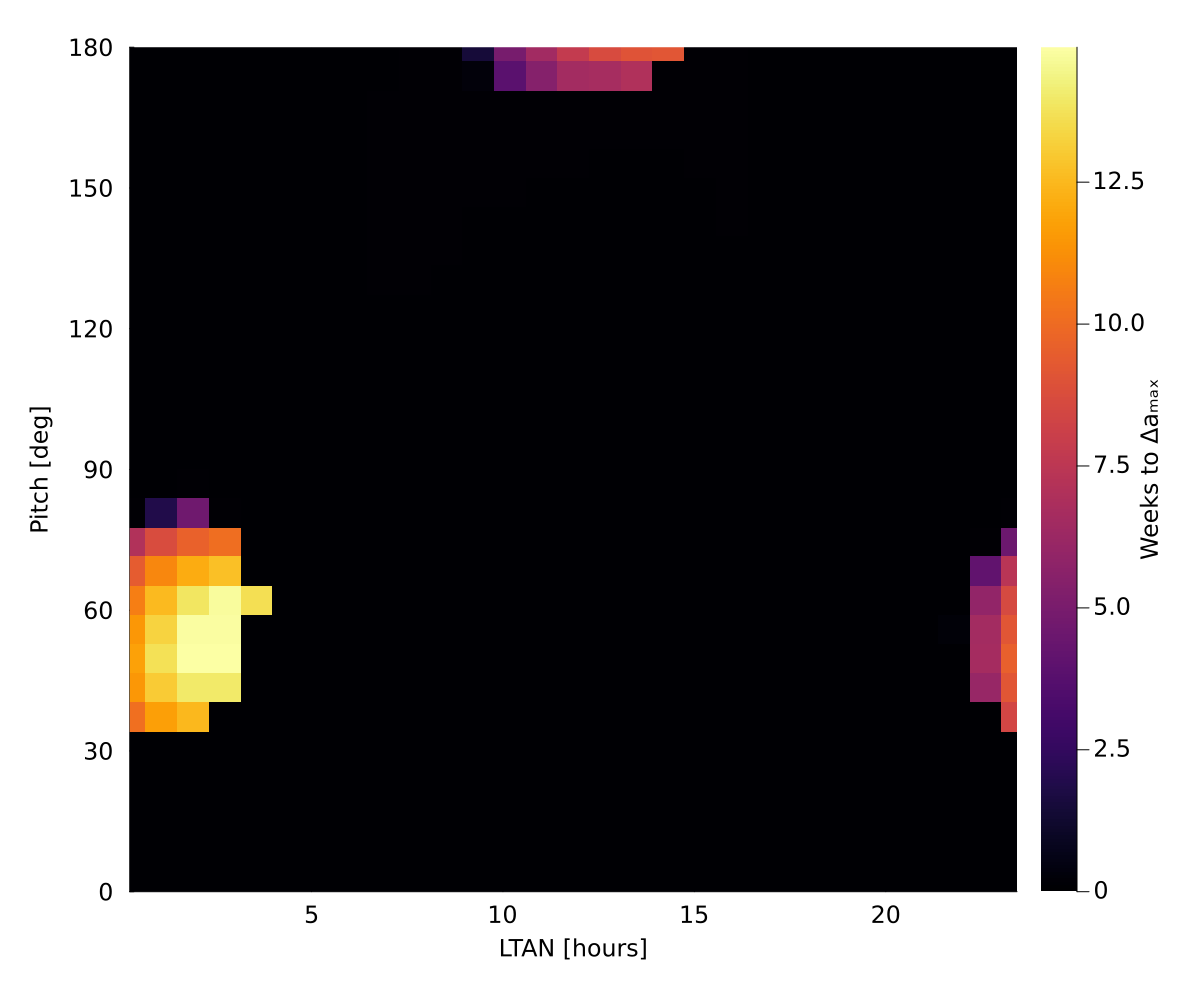
\includegraphics[width=1\linewidth]{figs/tmax_heatmap_ltan.png}
    \setlength{\abovecaptionskip}{0pt}
    \caption{Time taken for $\Delta a$ in search space}
    \label{fig:tmax}
\end{figure}

\par\noindent Almost all candidate solutions around the global maximum violate this empirical 3 month constraint. However all solutions in this space gain \( a \) continuously throughout the first 3 months. Hence this region of the set still holds the subset of candidate trajectories.

\vspace{5pt}
\par\noindent While the observed feathering behaviour appears to passively suppress out-of-plane perturbations and support quasi-steady SSO evolution, it is difficult to rigorously quantify the duration for which this condition can be maintained. In particular, modelling the residual out-of-plane SRP force in the feathered state is challenging, as napkin estimates indicate that the resulting acceleration lies close to machine precision limits. Consequently, the SRP-induced \( F_N \) component cannot be meaningfully captured in our current simulation framework. Moreover, the focus of this study is not to exhaustively characterize long-term SSO stability, but rather to demonstrate that significant \( a \) gain is achievable with a spin-stabilized, passively oriented sail. A more detailed treatment of long-duration quasi-steady SSO behavior, including effects such as attitude jitter, lateral area exposure, and precessional misalignment, is left for future work.


\section{Stratospheric Demonstrator Mission}
\label{bexus_section}
\noindent In addition to ground-based structural and deployment testing, the feasibility of solar sail deployment in a near-space environment was investigated as part of the BEXUS stratospheric balloon mission programme. The principal aim of this flight experiment was to assess the dynamic behaviour of spin-tensioned membrane deployment under near-vacuum and low-temperature conditions. It also acted as a stepping stone towards further missions, by validating and flight testing the various deployment mechanisms. A sail deployment mechanism was built, tested and launched aboard the BEXUS 34 mission, on Friday 4 October 2024, reaching an altitude of 27.2 km. The specifications of the deployer and it's operating conditions are given in Table \ref{tab:sail_deployer_specs}.

\begin{table}[h!]
\centering
\begin{tabular}{ll}
\hline
\textbf{Specification} & \textbf{Value} \\
\hline
Sail size (nominal) & 2.4 $\times$ 2.4 m square\\
Sail membrane & Mylar, 12 micron\\
Sail maximum spinning rate & 100 RPM\\
Hanging hub mass & 8 kg\\
Deployment gravity& 0.99 g\\
Deployment atmospheric pressure& 16 mbar\\
Deployment temperature& $-63\,^{\circ}\mathrm{C}$\\
\hline
\end{tabular}
\caption{Specifications of the sail deployer}
\label{tab:sail_deployer_specs}
\end{table}

\subsection{Experiment Architecture}
\noindent The overall mechanical design consisted of a hub suspended below the balloon gondola, allowing $360^{\circ}$ clearance for sail deployment. The hub had a static (relative to the gondola) upper section, which contained the electronic control systems (motor, burn wire mechanisms and sensors), and a lower section containing the sail membrane and deployable booms. The lower section was purely mechanical and connected to the upper plate via bearings, allowing relative rotation.  

\vspace{5pt}
\par\noindent Due to the constraints of an extremely low budget and short project timeframe, a number of novel solutions were developed in order to deploy and spin the sail membrane:

\vspace{5pt}
\par\noindent \textbf{Deployable Booms} - Four rollable booms were utilised as 'masts', which extended and supported the sail membrane once being unwound from their individual spools. These were of an unconventional design, each employing a pair of spring steel tapes (sourced from off the shelf tape measures) fitted inside a compliant sleeve manufactured from Kapton tape. These booms are heavier per unit length when compared to standard composite booms, yet successfully supported themselves and the sail membrane at a 2.2 metre cantilevered extension without issue.

\vspace{2pt}
\par\noindent\textbf{Anti-blooming Mechanism} - Blooming is a common issue with rollable booms, where friction on the outer surface of the spool prevents the boom tip from extending, causing the radius of the spool to increase as it unwinds without actually extending the boom. This leads to the mechanism jamming and the motor stalling. To prevent this, an original form of anti-blooming mechanism was fabricated which compressed the each spool in the radial direction (Figure \ref{fig:mechanical}).

\vspace{2pt}
\par\noindent\textbf{Clutch Mechanism} - A single motor was used for both boom deployment and sail spinning. To achieve this, a mechanical clutch was implemented, which was actuated using a custom burn-wire deployed pin pull mechanism. This locked the spool in a deployed state when actuated, such that the motor would act to spin the entire sail hub rather than unwinding the spools. The advantage of this system was that no slip rings were required for communication over rotary joints, as all electronics were mounted on the static portion of the hanging hub. A similar burn wire mechanism was used to both hold the sail compartment doors closed, and prevent rotation of the motor during the ascent.

\vspace{2pt}
\par\noindent\textbf{Cameras} - An array of cameras were used to fulfil the mission objective of investigating the spinning membrane dynamics. These were mounted beneath the balloon gondola, pointing at the sail deployer from various inclinations and directions. They were set to record at the beginning of the the deployment sequence, saving the footage to redundant sd cards mounted in the electronics box. One camera's stream of footage was also fed to the ground station for visual feedback during the deployment. The cameras recorded at 1 fps, 640x480 pixel resolution, in black and white. A key oversight of the mission planning was the lack of artificial illumination for the cameras to record the deployment and spinning of the sail.


\begin{figure}[H]
    \centering
    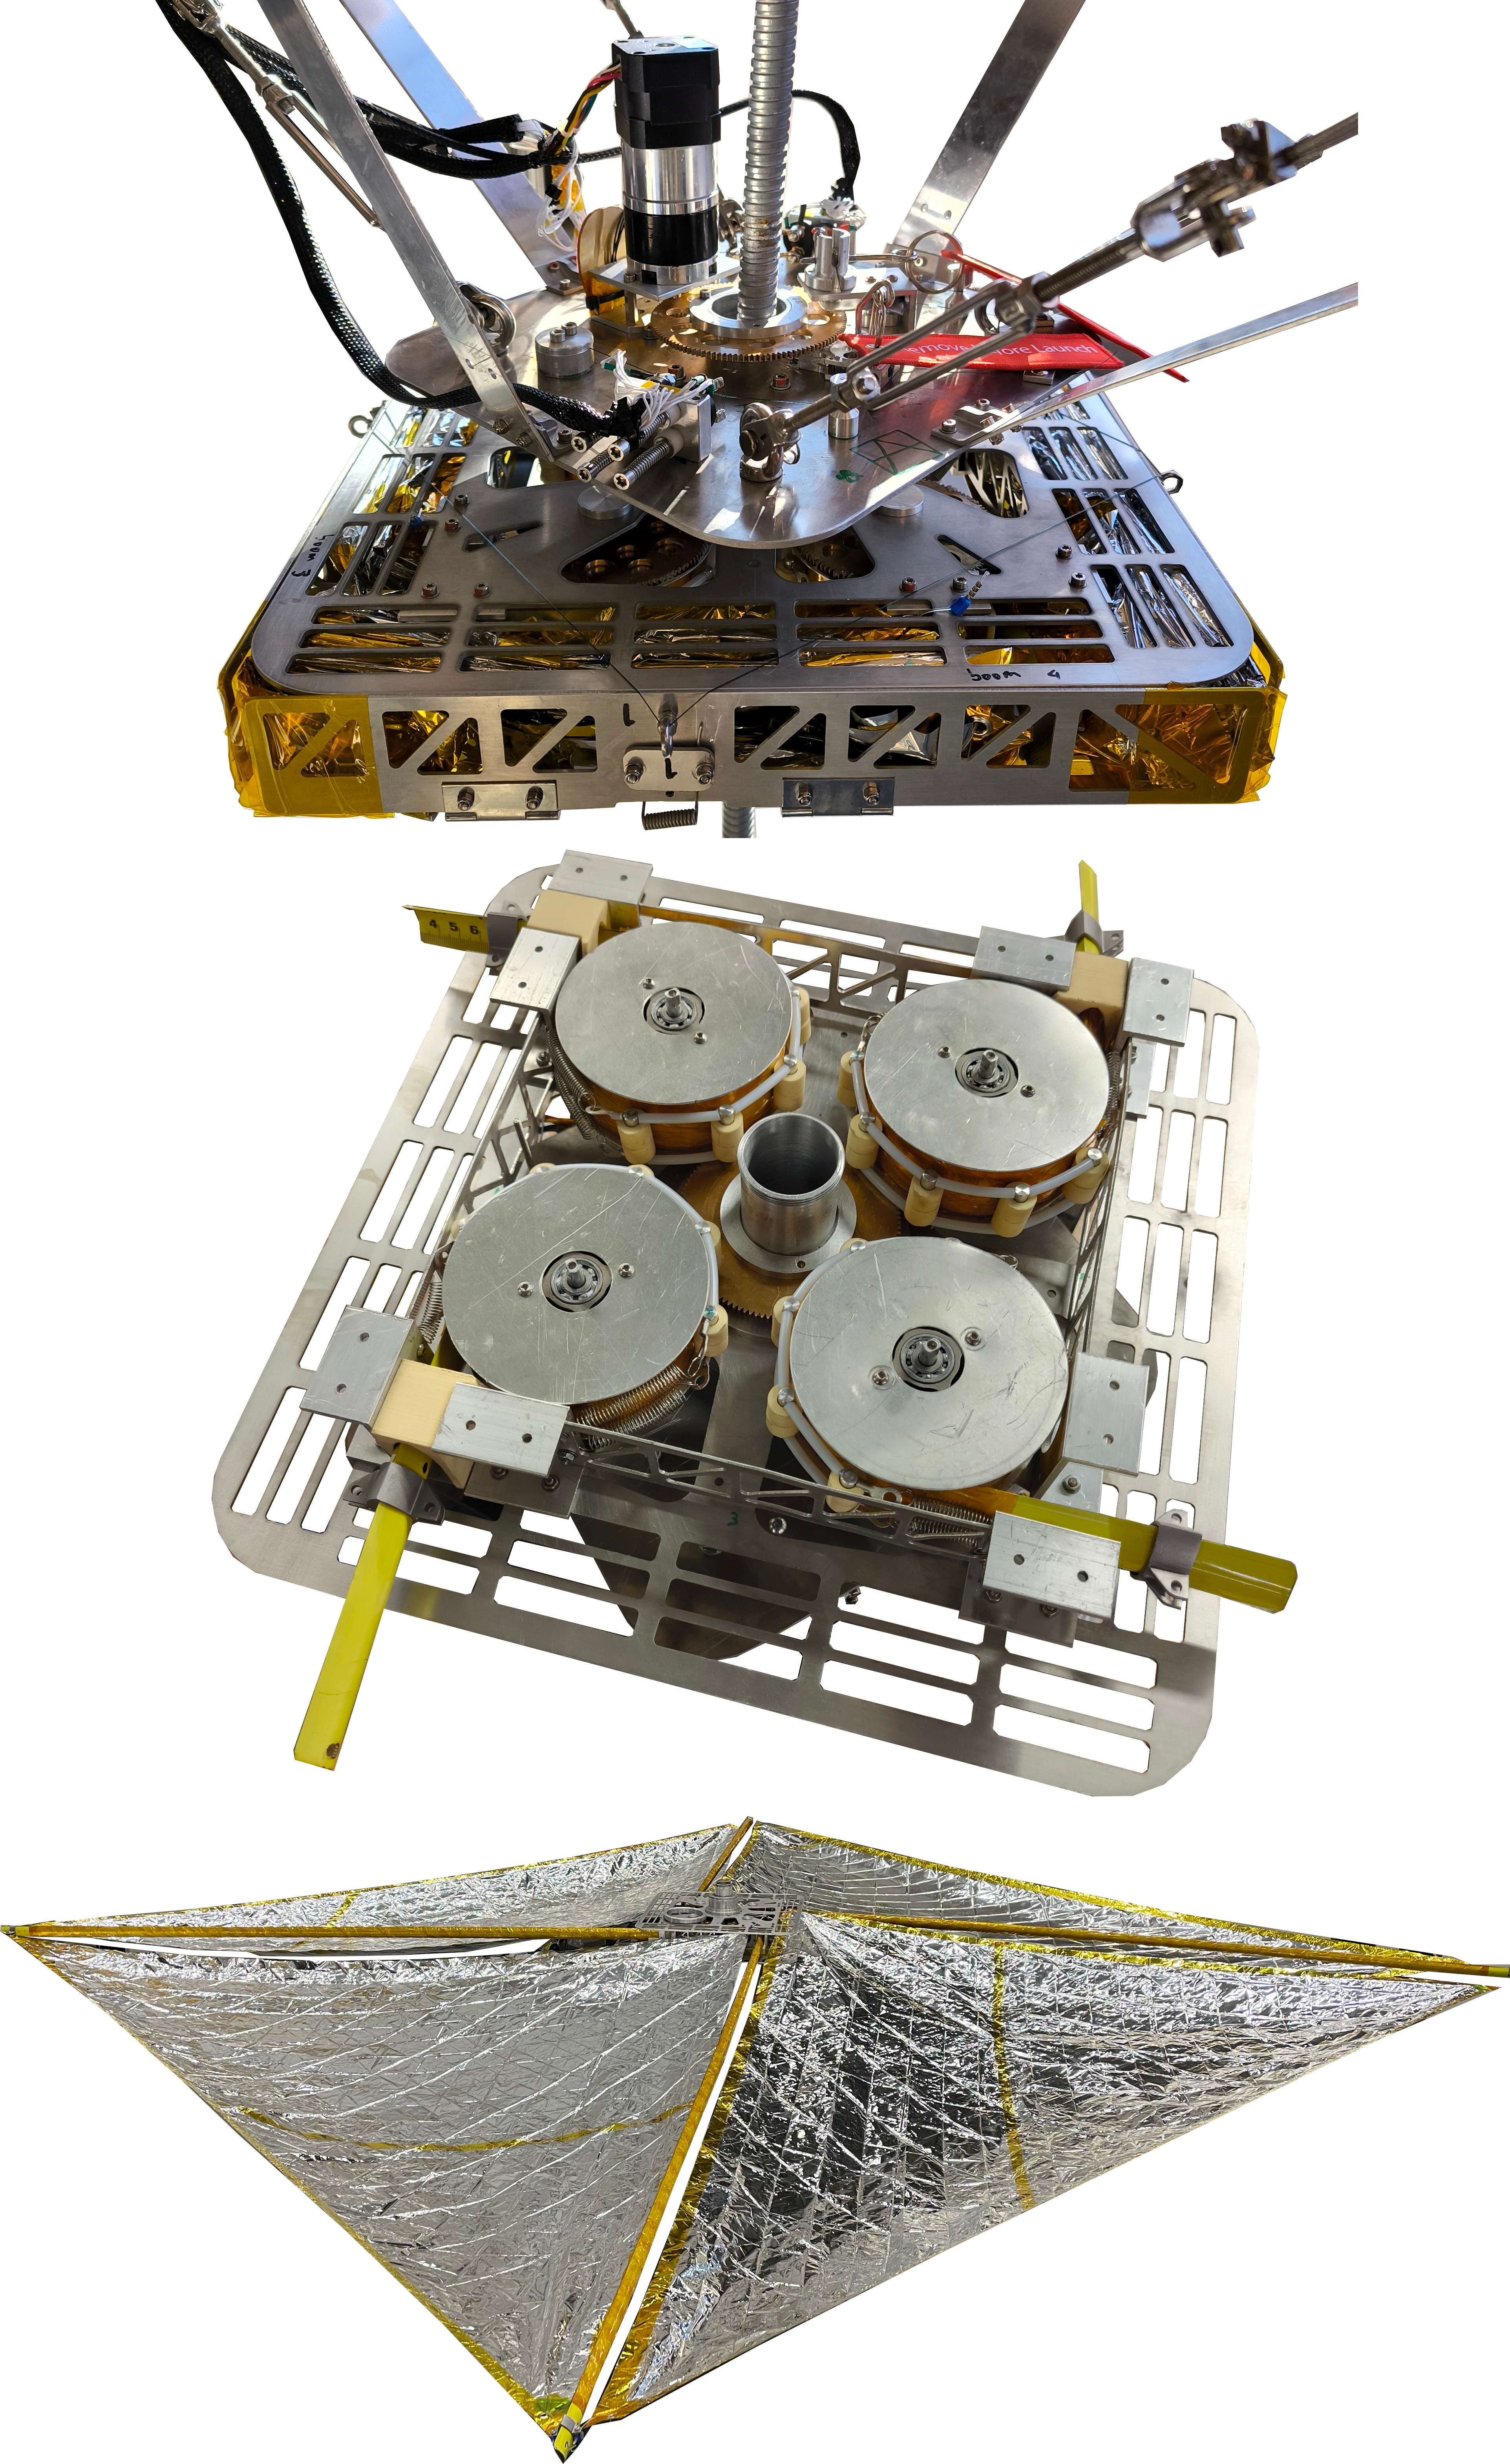
\includegraphics[width=1\linewidth]{figs/sail.jpg}
    \caption{Sail deployer - Upper: Sail deployer mechanism ready for flight, Middle: Boom spools and anti-blooming chains (underside of sail hub), Lower: Deployed sail}
    \label{fig:mechanical}
\end{figure}

\vspace{2pt}
\par\noindent\textbf{Communication} - The BEXUS balloon utilises an 'E-Link' antenna hanging below the gondola in order to facilitate communication between the balloon and the ground station. Due to the placement of the experiment below the balloon gondola, the sail deployer mechanism was designed with a 35 mm diameter hole through the centre. This requirement had the effect of enlarging the concentric shafts and bearings used for the deployment drive shaft and the sail spinning shaft.

\vspace{5pt}
\par\noindent A benefit of the balloon launch over equivalent rocket launched missions (for example the REXUS programme) is the ability to manually control the deployment sequence with real time feedback. This allowed for more flexibility if the mechanism malfunctioned. Due to limited bandwidth, a single frame from one of the cameras was sent to the ground station every 30 seconds during the experiment. Further measurements from the Svarog experiment was sent to the ground station during the flight, including motor RPM, accelerometer data from the hanging sail deployer, and electrical information. Telemetry from the gondola itself was also recorded, including position, speed, altitude and temperature.


\vspace{5pt}
\par\noindent\textbf{Sail Folding} - In order to unfurl the sail quadrants in a safe manner which both imparts minimal stress to the sail while also minimising volume within the sail hub body, the sail must be folded in a specific pattern. For the BEXUS 34 launch campaign, we chose to follow a horizontal-to-vertical zig-zag folding method which compacted each sail (right angle triangle of dimensions 3.1 x 2.1 x 2.4 m) into a rectangular block of dimensions 0.3 x 0.05 x 0.07 m (width x height x depth).

\vspace{5pt}
\par\noindent The folding procedure is shown in Figure \ref{fig:sail_folding}. The general procedure involves defining a central axis on each sail which connects the vertex of the two shortest sides (the vertex which connects to the central hub) to the point on the longest edge at a 90° angle. This allows us to define the horizontal axis as along the longest edge of the sail, and the vertical axis as being along this central axis. The sail is first folded along the horizontal axis from the outer vertices to the inward central axis, and then the sail is folded vertically in a zig-zag pattern to minimise stress on the folded joints when unfurling the sail. 

\begin{figure}[htbp]
    \centering
    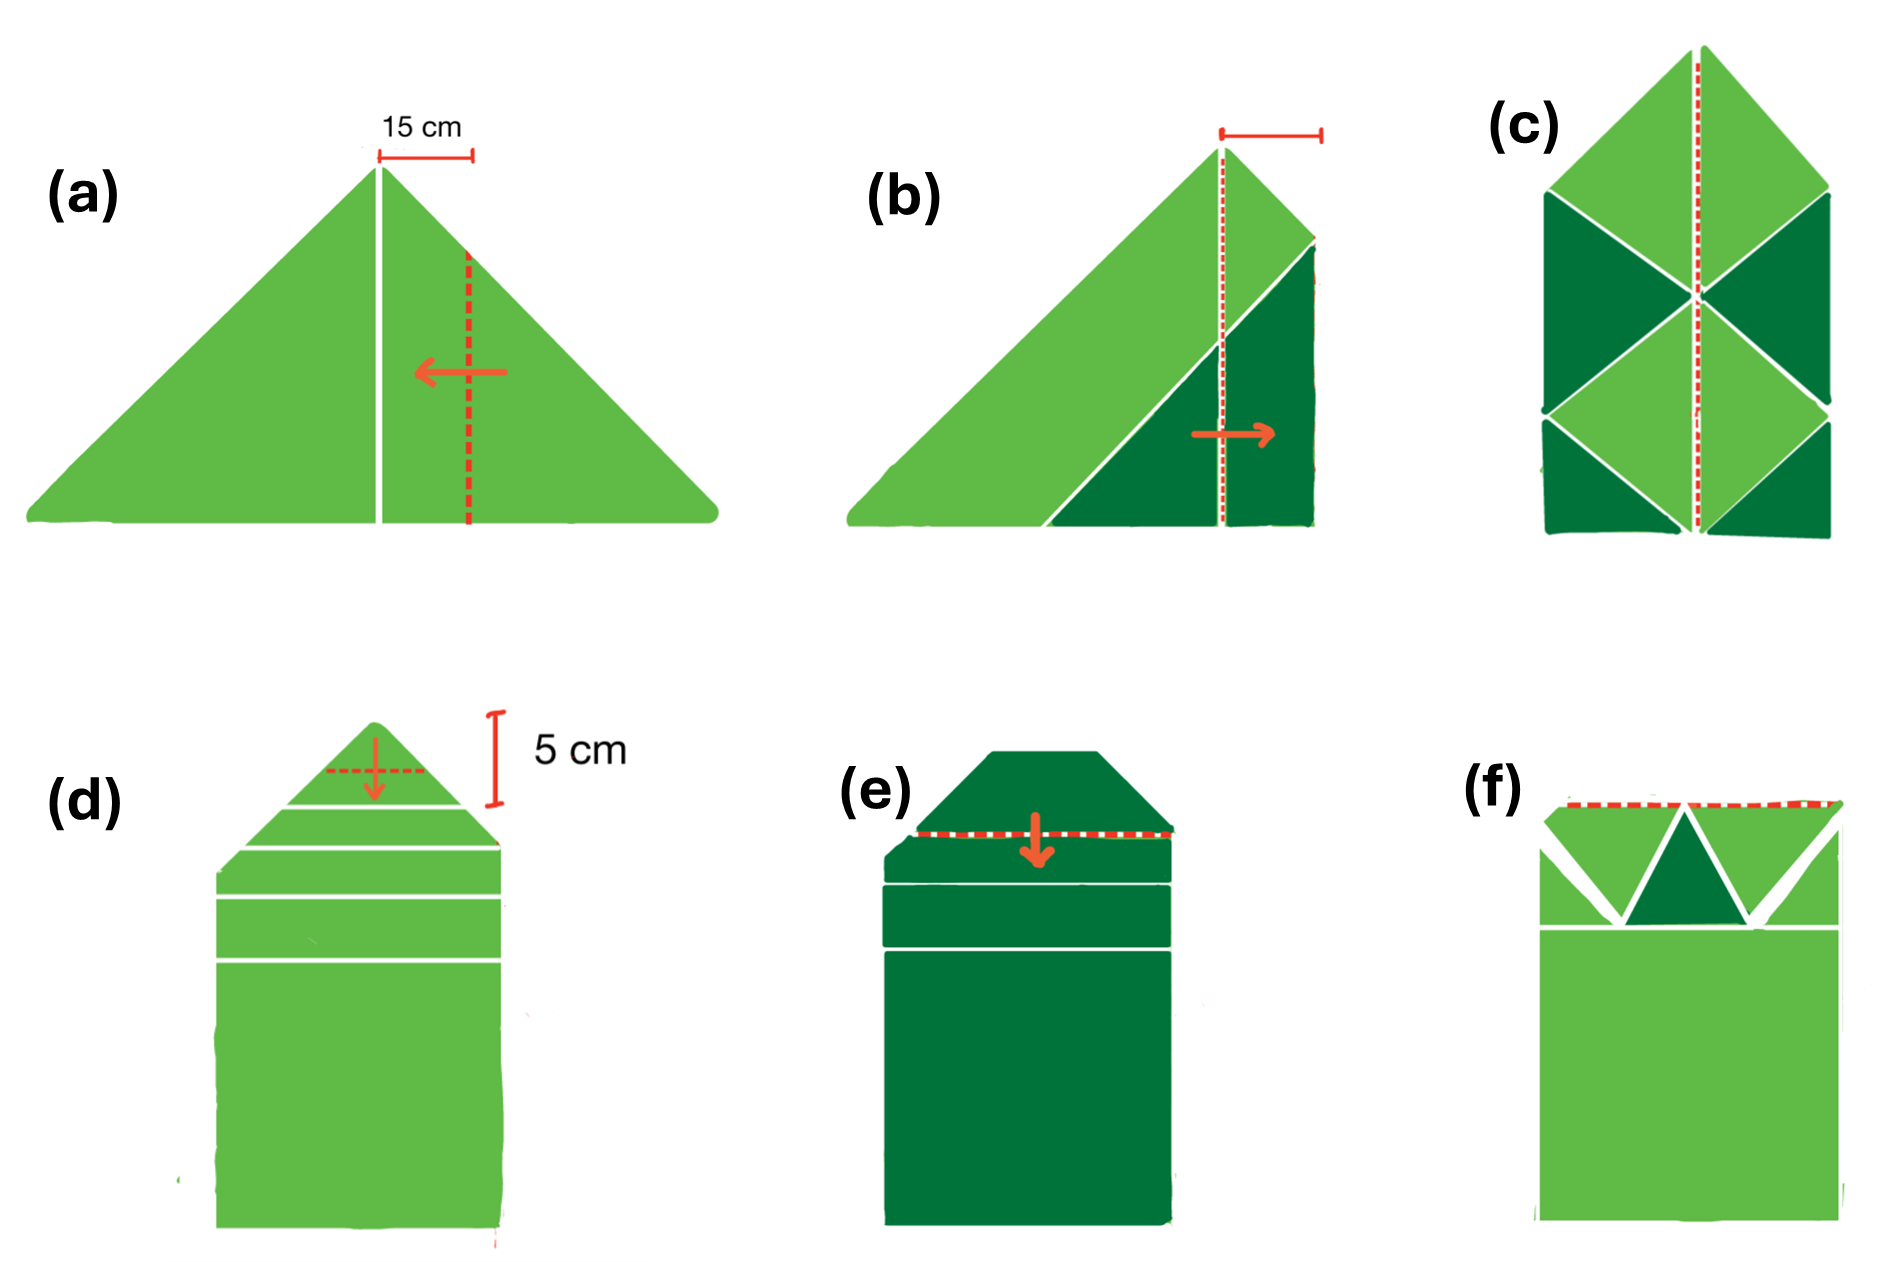
\includegraphics[width=1\linewidth]{figs/sail_folding_isss.png}
    \caption{Illustration of the sail folding procedure}
    \label{fig:sail_folding}
\end{figure}
\vspace{7pt}
\subsection{Electronics Overview}

\noindent An electronics box mounted inside the gondola housed the Main Processing Board (MPB). This contained the main and secondary processing units, which were a Raspberry Pi Model 3 and four Raspberry Pi Zeros, respectively. The components inside the electronics box interfaced with external components via 7 interconnects, five of which were custom PCBs. Connections were made in this way to isolate the electronics box for the sake of modular design, preventing damage to the internal circuitry and maintaining reliable connections.  

\vspace{5pt}
\par\noindent Effective and reliable motor systems were essential for the success of the launch. A B-G431B-ESC motor board drove the Brushless DC (BLDC) motor responsible for the deployment and spinning of the sail. The board interfaced via UART with the main MPU and used the 24V supply from the motor current limiting board to drive an RS Pro 8-pole, 3-phase BLDC motor drawing 1.79A. The motor control board software also handled communication between the motor control system and the main processing unit of the craft.  
\vspace{7pt}
\subsection{Testing and Flight}
\noindent Prior to launch, the full assembly and electronics underwent a Thermal Vacuum (TVAC) test, along with static load tests and a series of ground-based integration and communication trials. These validated the experiment for flight readiness.

\vspace{5pt}
\par\noindent During the BEXUS 34 mission, solar sail deployment began as planned but was impeded when two compartment doors opened only partially (Figure \ref{fig:flight}). This caused two booms to catch, jamming the deployment. The spin-up sequence was initiated in an attempt to release the booms via centrifugal force, but it was unsuccessful. Although some sail material unfurled due to spinning, full deployment was not achieved. Post-flight inspection confirmed that the door spring-hinge assembly was at fault for the failure, providing a valuable learning opportunity for the mechanical sub-team.

\begin{figure}[htbp]
    \centering
    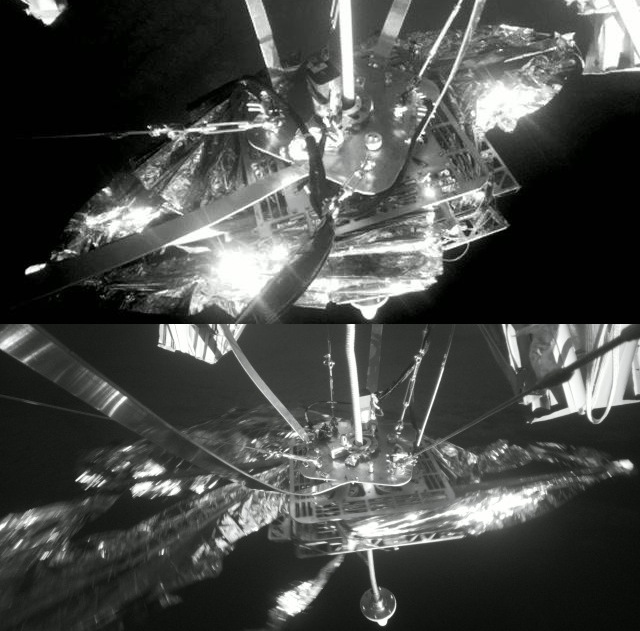
\includegraphics[width=1\linewidth]{figs/flight.jpg}
    \caption{Flight footage - Upper: Deployment malfunction, Lower: Spinning}
    \label{fig:flight}
\end{figure}

\noindent Operational constraints during flight further complicated the situation. The launch had been delayed by poor weather, pushing sail deployment close to sunset. This created harsh lighting conditions and limited visual feedback from the downlink camera. The risk of total darkness, which would eliminate all visual telemetry, contributed to time pressure and prompted a slightly rushed response to the door malfunction.

\vspace{5pt}
\par\noindent Critically, no procedures had been developed for reversing a partial deployment by rewinding the booms—a potential recovery action that might have cleared the jammed doors and enabled full opening. This exposed a shortfall in contingency planning and test coverage.

\vspace{5pt}
\par\noindent Despite these setbacks, the mission yielded important insights for future flights, including the need for improved hinge mechanisms, real-time feedback systems, and validated recovery procedures for partial deployment scenarios.
\vspace{7pt}
\subsection{Data processing}
\noindent In the event of a fully successful deployment, the plan was to analyse the solar sail’s dynamics and reconstruct its geometry using visual data from onboard cameras. This method, inspired by JAXA’s approach \citep{ikaros_shape}  for IKAROS, relies on photometric shape reconstruction. Assuming the Sun as a planar light source, variations in brightness correspond to surface angles, enabling geometric inference—provided the membrane has low curvature gradients.

\vspace{5pt}
\par\noindent The first step involved detecting the sail’s edges using OpenCV’s edge detection algorithms to isolate the aluminized regions. However, due to the failed deployment and resulting high curvature, the reconstruction proved infeasible. Standard inverse ray tracing methods could not handle the complex geometry. Future efforts may explore advanced non-linear fitting techniques, though success is uncertain. With a proper deployment and smoother surface, the current algorithm is expected to perform as intended.

\vspace{5pt}
\par\noindent A separate approach was tested using 3D reconstruction techniques from the camera footage. These were based on either photogrammetric reconstruction, using MeshRoom \citep{alicevision2021} software, or Neural Radiance Fields (NeRFs) which could then be converted into a mesh body (using Instant-NGP). However, it was found that due to the low resolution and limited number of camera angles, along with poor lighting conditions, these techniques had limited success. Notably, the NeRF method was much more capable of understanding the reflective surface of the Mylar membrane (compared to photogrammetry), showing real promise when the number of cameras and their resolution was increased in ground testing. 

\vspace{5pt}
\par\noindent In order to facilitate 3D reconstruction of the sail membrane in the future, a larger array of cameras (at least 10 angles) could be implemented, controlled with synchronised shutters and a low exposure time (to minimise motion blur). Depending on the stability of the membrane geometry, an alternative would be to use a smaller line array of cameras to scan the spinning sail from one direction at multiple inclinations - similarly to how commercial scanners use a turntable to move the subject, rather than surrounding with cameras from all directions.

\vspace{7pt}
\section{Further Steps}
\subsection{BEXUS 36}
\noindent Project Svarog has been accepted to launch a sail deployment mechanism aboard BEXUS 36 in October 2025. The aim of the mission is once again to assess the dynamic behaviour of spin-tensioned membrane deployment under near-vacuum and low-temperature conditions. Learnings from the failures of the BEXUS 34 launch are being implemented into a completely redesigned hub, with certain subcomponents carried over (i.e. the Kapton-tape-spring booms, sail spinning motor, gondola mounted electronics box and cameras). A secondary objective of the mission is to compress the mechanism into a smaller package that would more closely match a LEO orbiter. To this end, an 8 unit cubesat form factor has been selected (approximately a 200 x 200 x 200 mm cube), using a single spool for all four booms (improving packing efficiency compared to the BEXUS 34 launch).

\begin{figure}[htbp]
    \centering
    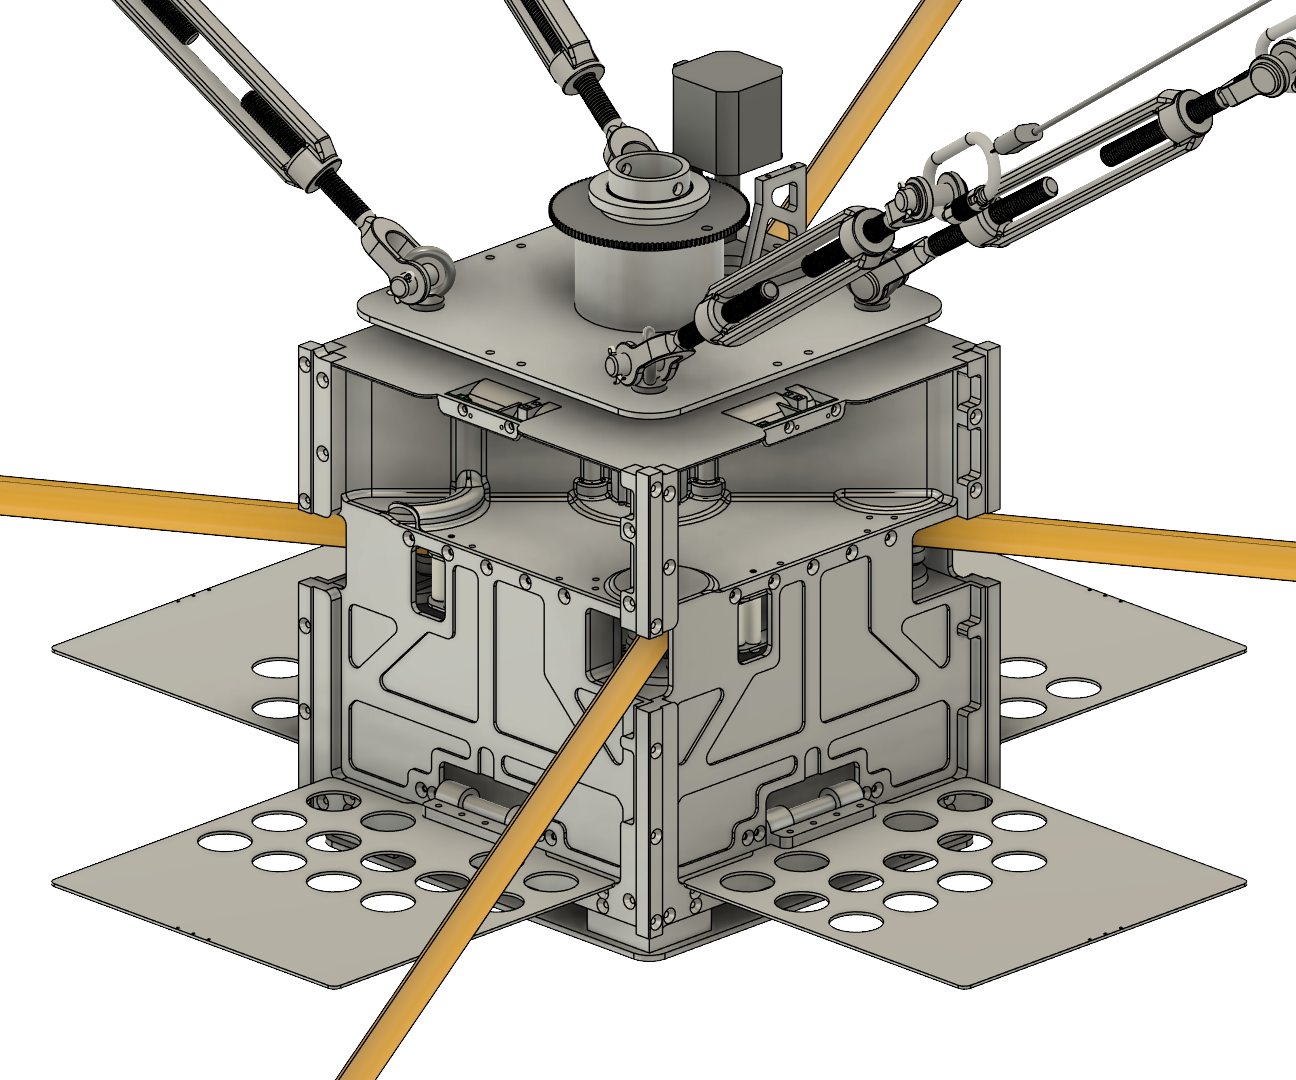
\includegraphics[width=1\linewidth]{figs/02 Integration Assembly v43.png}
    \caption{BEXUS 36 Cubesat (sail compartment doors and booms deployed) and Interface Plate}
    \label{fig:BX36}
\end{figure}

\noindent The Cubesat will be mounted below an interface plate (attached to the gondola) which controls the rotation of the entire Cubesat for sail spinning. In an orbital mission, there would be no interface plate to react against, and as such an internal reaction system would be required in the Cubesat. Thus the tertiary objective of the BEXUS 36 launch will be to validate the spin up and ejection of a reaction wheel, which would be used in orbit to initiate spinning of the Cubesat. To simplify this objective, the reaction wheel has been reduced in mass and RPM for the BEXUS 36 launch, such that it will not serve to spin the Cubesat via reaction, but rather simply validate the mechanism.
\vspace{7pt}
\subsection{LEO mission}
\noindent Project Svarog's next major milestone after the completion of BEXUS 36 will be to build a prototype which will be ready for a LEO launch. Key changes between the BEXUS 36 demonstrator and a true LEO satellite will be the implementation of composite booms, an internal power and communications system, and attitude control. 

\vspace{5pt}
\par\noindent The orbital simulations we would need to run can be handled by the code described in this paper. The exact orbit will depend on the LEO program we eventually apply for. An orbit in the range of 600-800km in altitude for 6 months or more in SSO would be ideal to minimise drag and test the impact of solar radiation propulsion. However, we would still be able to complete a valuable test at lower altitudes.

\section{Conclusions}
\noindent The developments made by the Project Svarog team over the last two years has been significant in both of its core working groups. In this paper we highlighted the improvements made to the in-house orbital simulation code developed for simulating test LEO orbits and future interplanetary trajectories, as well as developments made in our mechanical prototyping.

\vspace{5pt}
\par\noindent From our orbital simulations, we can say that we have high confidence in attitude stability over 30 days (thus we can meet primary objective of data collection, spin up, boom deployment and more). Furthermore, if we manage to get a desirable launch timing we could potentially show an increase in SMA  but it requires an optimal launch LTAN and altitude of 600 km or greater, but long term attitude stability and SSO perturbation needs to be studied with greater fidelity (and ideally we can get better sail loading).

\vspace{5pt}
\par\noindent Regarding the mechanical integration progress, BEXUS 36 is providing us the perfect platform to develop our technology into a more CubeSat-like form-factor which we hope will allow us to gain further flight heritage on our mechanisms and experience in developing real flight-hardware. In the next 2-3 years, we hope to be selected to fly as a secondary payload on a LEO launch which can send our solar sail CubeSat to space where we will be able to test both our orbital simulations and existing flight-hardware in a real space environment.

\section*{Acknowledgements}
\noindent The authors of this paper thank our academic supervisors, Dr. Aaron Knoll and Professor Matthew Santer, for their advice and support of our team over the years. We also acknowledge the contributions of REXUS/BEXUS programme and the associated space agencies that help run it (See statement below*) - providing a platform to build and test our first ever mechanical prototype has been an invaluable contribution. The authors also thank the REXUS/BEXUS program manager, Esmée Menting, and our mentor for the project, Dr. Dorota Budzyn. Moreover, the following members, despite not having been involved in this paper, have provided invaluable contributions to the team’s design effort during the past year (in alphabetical order): Gil Barbosa Ribeiro, Ivan Revenga Riesco, Golf Rojnuckarin, Beatriz Soriano Tortosa. Finally, we thank Imperial College London for providing funding and facilities for us to build, test and integrate our designs.

\vspace{5pt}
\par\noindent *The REXUS/BEXUS programme is realised under a bilateral Agency Agreement between the German  Aerospace  Center  (DLR)  and  the  Swedish  National  Space  Agency  (SNSA).  The Swedish  share  of  the  payload  has  been  made  available  to  students  from  other  European countries  through  a  collaboration  with  the  European  Space  Agency  (ESA).  EuroLaunch,  a cooperation  between  the  Swedish  Space  Corporation  (SSC)  and  the  Mobile  Rocket  Base (MORABA) of DLR, is responsible for the campaign management and operations of the launch vehicles. Experts from DLR, SSC, ZARM and ESA provide technical support to the student teams  throughout  the  project.  REXUS  and  BEXUS  are  launched  from  SSC,  Esrange  Space Center in northern Sweden.

%%\section*{References}

%% If you have bibdatabase file and want bibtex to generate the
%% bibitems, please use
%%

\begin{nolinenumbers}

\bibliography{isss.bib}

\end{nolinenumbers}

%% else use the following coding to input the bibitems directly in the TeX file.

%% \begin{thebibliography}{00}

%% \bibitem{label}
%% Text of bibliographic item

%% \bibitem{}

%% \end{thebibliography}


\end{document}
\endinput

